\documentclass[a4paper,
fontsize=11pt,
%headings=small,
oneside,
numbers=noperiodatend,
parskip=half-,
bibliography=totoc,
final
]{scrartcl}


\usepackage[babel,maxlevel=3]{csquotes}
\usepackage{synttree}
\usepackage{graphicx}
\setkeys{Gin}{width=.4\textwidth} %default pics size

\graphicspath{{./plots/}}
\usepackage[ngerman]{babel}
\usepackage[T1]{fontenc}
%\usepackage{amsmath}
\usepackage[utf8x]{inputenc}
\usepackage [hyphens]{url}
\usepackage{booktabs} 
\usepackage[left=2.4cm,right=2.4cm,top=2.3cm,bottom=2cm,includeheadfoot]{geometry}
\usepackage[labelformat=empty]{caption} % option 'labelformat=empty]' to surpress adding "Abbildung 1:" or "Figure 1" before each caption / use parameter '\captionsetup{labelformat=empty}' instead to change this for just one caption
\usepackage{eurosym}
\usepackage{multirow}
\usepackage[ngerman]{varioref}
\setcapindent{1em}
\renewcommand{\labelitemi}{--}
\usepackage{paralist}
\usepackage{pdfpages}
\usepackage{lscape}
\usepackage{float}
\usepackage{acronym}
\usepackage{eurosym}
\usepackage{longtable,lscape}
\usepackage{mathpazo}
\usepackage[normalem]{ulem} %emphasize weiterhin kursiv
\usepackage[flushmargin,ragged]{footmisc} % left align footnote
\usepackage{ccicons} 
\setcapindent{0pt} % no indentation in captions
\usepackage{xurl} % Breaks URLs

%%%% fancy LIBREAS URL color 
\usepackage{xcolor}
\definecolor{libreas}{RGB}{112,0,0}

\usepackage{listings}

\urlstyle{same}  % don't use monospace font for urls

\usepackage[fleqn]{amsmath}

%adjust fontsize for part

\usepackage{sectsty}
\partfont{\large}

%Das BibTeX-Zeichen mit \BibTeX setzen:
\def\symbol#1{\char #1\relax}
\def\bsl{{\tt\symbol{'134}}}
\def\BibTeX{{\rm B\kern-.05em{\sc i\kern-.025em b}\kern-.08em
    T\kern-.1667em\lower.7ex\hbox{E}\kern-.125emX}}

\usepackage{fancyhdr}
\fancyhf{}
\pagestyle{fancyplain}
\fancyhead[R]{\thepage}

% make sure bookmarks are created eventough sections are not numbered!
% uncommend if sections are numbered (bookmarks created by default)
\makeatletter
\renewcommand\@seccntformat[1]{}
\makeatother

% typo setup
\clubpenalty = 10000
\widowpenalty = 10000
\displaywidowpenalty = 10000

\usepackage{hyperxmp}
\usepackage[colorlinks, linkcolor=black,citecolor=black, urlcolor=libreas,
breaklinks= true,bookmarks=true,bookmarksopen=true]{hyperref}
\usepackage{breakurl}

%meta
%meta

\fancyhead[L]{T. Steiner\\ %author
LIBREAS. Library Ideas, 44 (2023). % journal, issue, volume.
\href{https://doi.org/10.18452/28264}{\color{black}https://doi.org/10.18452/28264}
{}} % doi 
\fancyhead[R]{\thepage} %page number
\fancyfoot[L] {\ccLogo \ccAttribution\ \href{https://creativecommons.org/licenses/by/4.0/}{\color{black}Creative Commons BY 4.0}}  %licence
\fancyfoot[R] {ISSN: 1860-7950}

\title{\LARGE{\enquote*{Alte Traditionen}: zur Rolle von scholar-led publishing und Open Access in den Geistes- und Sozialwissenschaften}}% title
\author{Tobias Steiner} % author

\setcounter{page}{1}

\hypersetup{%
      pdftitle={`Alte Traditionen': zur Rolle von scholar-led publishing und Open Access in den Geistes- und Sozialwissenschaften},
      pdfauthor={Tobias Steiner},
      pdfcopyright={CC BY 4.0 International},
      pdfsubject={LIBREAS. Library Ideas, 44 (2023).},
      pdfkeywords={Diamond Open Access, scholar-led, Publikationsmarkt, Wissenschaftskommunikation, wissenschaftsgeleitetes Publizieren, Open Access},
      pdflicenseurl={https://creativecommons.org/licenses/by/4.0/},
      pdfurl={https://doi.org/10.18452/28264},
      pdfdoi={10.18452/28264},
      pdflang={de},
      pdfmetalang={de}
     }



\date{}
\begin{document}

\maketitle
\thispagestyle{fancyplain} 

%abstracts
\begin{abstract}
\noindent
\textbf{Kurzfassung}: Der vorliegende Beitrag beleuchtet den Ansatz des
scholar-led publishing und zeigt auf, welche Zusammenhänge zwischen
scholar-led Initiativen und der \enquote*{klassischen} Open Access-Bewegung
bestehen. Nach einer kurzen Diskurseinordnung leitet der Beitrag
diachron ab, wie scholar-led Initiativen aus den Geistes- und
Sozialwissenschaften schon früh und parallel zu den weithin rezipierten
Entwicklungen aus dem medizinisch-naturwissenschaftlichen Bereich der
1990er Jahre auf eigene Weise wichtige Impulse zur Öffnung von
Publikationskulturen setzten. Dazu werden exemplarisch eine Vielzahl von
medien- und kulturwissenschaftlichen scholar-led Journals, Buchverlagen
sowie weiterreichenden Netzwerk- und Infrastruktur-Initiativen entlang
der größeren Entwicklungen der letzten vier Jahrzehnte hin zur
Digitalisierung von wissenschaftlichen Publikationspraktiken und dem
sich daraus ergebenden Potential eines alternativen Publikationssystems,
welches gemeinschaftliche Kollaboration unter den Vorzeichen von
Gemeinnützigkeit über kommerzorientierten Wettbewerb stellt.
\end{abstract}

%body
Publikationskulturen sind im Wissenschaftsbetrieb ähnlich vielfältig wie
die ihnen zugrundeliegenden Forschungskulturen. Im heutzutage oftmals
normativ geführten Diskurs um Open Access besteht die Gefahr, dass diese
Vielfalt zugunsten techno-solutionistischer Implementationen ins
Hintertreffen gerät oder gar mittelfristig verloren geht. Der
vorliegende Beitrag geht im Folgenden daher näher auf den Ansatz des
\textbf{scholar-led publishing} ein und zeigt auf, welche Zusammenhänge
zwischen scholar-led-Initiativen und der \enquote*{klassischen}
Open-Access-Bewegung bestehen.

Dazu beginne ich mit einer kurzen Begrifflichkeits- und
Diskurseinordnung und leite dann diachron ab, wie scholar-led
Initiativen aus den Geistes- und Sozialwissenschaften -- und mit ihnen
aus den Kultur-, Medien- und Kommunikationswissenschaften -- schon früh
und parallel zu den weithin rezipierten Entwicklungen aus dem
medizinisch- naturwissenschaftlichen Bereich der 1990er Jahre auf eigene
Weise wichtige Impulse zur Öffnung von Publikationskulturen setzten.
Darauf folgend stelle ich ein Spektrum von scholar-led
Journal-Initiativen, Buchverlagen sowie scholar-led Netzwerken und
Kollaborationen im weiteren Sinn vor.\footnote{Teile des vorliegenden
  Beitrags wurden 2022 als Blog-Dreiteiler im Open-Media-Studies-Blog
  der Zeitschrift für Medienwissenschaften (Teile 1, 2, 3)
  veröffentlicht:

  Teil 1:
  \url{https://zfmedienwissenschaft.de/online/open-media-studies-blog/pluralities-scholar-led-publishing-und-open-access}

  Teil 2:
  \url{https://zfmedienwissenschaft.de/online/open-media-studies-blog/old-traditions-scholar-led-publishing-und-open-access}

  Teil 3:
  \url{https://zfmedienwissenschaft.de/online/open-media-studies-blog/new-communities-scholar-led-publishing-und-open-access}}

\hypertarget{scholar-led-open-access-genealogien-im-digitalen-raum}{%
\section{scholar-led \& Open Access: Genealogien im digitalen
Raum}\label{scholar-led-open-access-genealogien-im-digitalen-raum}}

Einleitend sei zu erwähnen, dass sowohl \enquote*{Open Access} als auch
\enquote*{scholar-led publishing} im Folgenden im Sinne von Samuel Moore
als \emph{boundary objects} verstanden werden. Moore überträgt Susan
Leigh Stars und James Griesemers Konzeption des \emph{boundary object}
(1989) als \enquote{concept that has a specific understanding in a local
community of practice but is rigid enough to maintain its definition
across communities} (\href{https://doi.org/10.4000/rfsic.3220}{2017}) in
den Open-Access-Kontext und zeigt auf, dass die oftmals im Diskurs als
einheitlich dargestellte \enquote*{Bewegung} um Open Access tatsächlich
eine Vielzahl verschiedener Ursprünge, damit einhergehender
Motivationen, sowie daraus resultierender, variierender Interpretationen
und sich entwickelnder Praktiken in sich trägt. Moore nennt hier
beispielsweise Einflüsse \enquote{from the formalising of pre-existing
preprint cultures via subject repositories and the emergence of
institutional repositories, to the free culture and open-source software
movements} (\href{http://journals.openedition.org/rfsic/3220}{2017}) und
konstatiert zusammenfassend, dass der Minimalkonsens zwischen den
einzelnen Open-Access-Strömungen wohl darin bestehe, dass
Forschungsergebnisse in irgendeiner Art frei zugänglich im Web verfügbar
gemacht werden sollen.

\hypertarget{zum-begriff-scholar-led}{%
\subsection{\texorpdfstring{Zum Begriff
\enquote*{scholar-led}}{Zum Begriff `scholar-led'}}\label{zum-begriff-scholar-led}}

Als einer der wichtigen Einflüsse, dessen Ursprünge, Motivationen und
Praktiken später auch in der Open-Access-Bewegung wiederkehren, kann
hier insbesondere der des unabhängigen scholar-led publishing gesehen
werden. Mit dem Adjektiv \emph{scholar-led}\footnote{Oftmals wird auch
  \emph{academic-led} quasi synonym verwendet, allerdings bestehen hier
  definitorische Unterschiede, da das Adjektiv \enquote{academic-led}
  Wissenschaftler*innen mit einer bestehenden institutionellen Bindung
  bezeichnet, während \enquote{scholar-led} inklusiver auch
  Wissenschaftler*innen mit einschließt, die beispielsweise keine
  direkte Affiliation innehaben oder beruflich in anderen Bereichen,
  aber dennoch entweder darüber oder in ihrer Freizeit im
  wissenschaftlichen Ökosystem tätig sind.\\
  Dies war nebenbei auch der ausschlaggebende Grund bei der Namenswahl
  des \href{https://scholarled.org}{ScholarLed}-Konsortiums 2018. Siehe
  dazu auch Adema und Stone,
  \href{https://repository.jisc.ac.uk/6666/1/Changing-publishing-ecologies-report.pdf}{Changing
  Publishing Ecologies,} 2016, Fathallah, 2023, oder Steiner, 2023.}
werden Initiativen bezeichnet, die in verschiedenen Ausprägungen der
Wissenschaftskommunikation betrieben werden -- primär durch im
Wissenschaftsbetrieb beschäftigte Personen, die dies hauptsächlich in
ihrer Freizeit neben oder teilweise im Kontext ihrer Hauptanstellung im
Wissenschaftssystem hauptverantwortlich übernehmen. In
konstruktiv-integrativ gedachter Konnotation schließt der Begriff
der/des \emph{scholars} hier neben Forschenden mit institutioneller
Anbindung auch explizit Forschende ohne institutionelle Affiliation
sowie weitere im Wissenschaftsbetrieb tätige Personengruppen, zum
Beispiel Lehrende, Bibliothekar*innen, Mitarbeitende aus
wissenschaftsunterstützenden Bereichen (Projektkoordination, e-Learning,
IT, et cetera), als auch Promovierende und Studierende in höheren
Semestern mit ein, sofern diese aus einer Position des \emph{independent
scholars} heraus agieren und nicht die möglicherweise parallel
hauptberuflich ausgefüllte offiziellen Rolle des/der Vertreter*in von
Institutionen in den Vordergrund tritt. Letztere würden sonst eher den
spezifischen Teilbereichen des institutionellen Publishings zugeordnet
werden (also in der Rolle des/der Vertreter*in einer Bibliothek dann
\emph{\enquote*{library-led}}, als Vertreter*in einer
Forschungsgesellschaft dann \emph{\enquote*{association-led}}). Die leitende
Rolle, die das \enquote{-led} impliziert, verstehe ich zudem nach Samuel
Moore
(\href{https://www.samuelmoore.org/2019/10/24/open-by-whom-on-the-meaning-of-scholar-led/}{2019})
spezifischer als nicht nur das Verfassen und Schreiben von Beiträgen,
sondern auch selbst die Kontrolle über technische, organisatorische und
administrative Aspekte innehabend.

Während \emph{scholar-led} in diesem Beitrag primär als
neutral-deskriptives Adjektiv gedacht ist, kann zudem festgehalten
werden, dass sich zahlreiche scholar-led Initiativen und unabhängige
scholar-led Verlage im Handlungs- und Wertesystem sowie in ihrer
Arbeits- und Organisationsweise als Alternativen insbesondere zu großen,
voll professionalisierten, kommerziell agierenden und auf
Gewinnmaximierung angelegten \enquote*{klassischen} Verlagen
positionieren. Im Kontrast zu \enquote*{klassischen} Verlagen legen
viele unabhängige scholar-led Projekte, Initiativen und Verlage einen
Duktus des sich im Sinne einer aktiven Selbstermächtigung von
institutionellen Beschränkungen frei machenden Publizierens zugrunde.
Das spiegelt sich dann auch im Tätigkeitsfokus wider, der zumeist auf
den Akt eines von neoliberal-kapitalistischen Marktlogiken weitgehend
entkoppelten \enquote*{esoterischen}\footnote{Im Sinne von Stevan
  Harnads \emph{subversive proposal} (1994), in welchem Harnad
  scholarship im Kern als \enquote*{esoteric}, also als von
  \enquote*{von einigen Wenigen für einige Wenige produziert} und somit
  jenseits von neoliberal-kapitalistischer Marktlogik existierend
  beschreibt.} Publizierens zielt. Entlang dieser durch den Kontext in
den USA oder Großbritannien geprägten Lesart\footnote{Diese
  Interpretation von \emph{scholar-led} publishing basiert auf einem
  stetig wachsenden Forschungskorpus, siehe beispielsweise Adema \&
  Stone 2017, Adema \& Moore 2017, Moore 2019, Adema \& Moore 2021,
  Steiner 2022, Fathallah, 2023, und Steiner 2023 für zahlreiche
  Beispiele sowie Querschnittsanalysen der zugrundeliegenden
  Motivationen.} von scholar-led publishing wird in diesem Beitrag daher
nicht weiter auf den Bereich von formalisierten wissenschaftsgeleiteten
Organisationen in Form wissenschaftlicher Gesellschaften, Verbünde und
Akademien eingegangen, und auch Universitätsverlage fallen nicht unter
das im Folgenden angelegte Raster, da diese Organisationsformen anderen
Gegebenheiten und Dynamiken unterliegen, als dies für das unabhängig
agierende scholar-led Publikationswesen der Fall ist.\footnote{Die
  letztgenannten Organisationsformen ließen sich pragmatisch unter dem
  weitreichenderen Adjektiv \enquote*{institution-led} oder, noch weiter
  gefasst, als \enquote*{community-led} (im Sinne von \enquote{aus der
  akademischen Community heraus}) subsumiert werden -- siehe hier
  beispielsweise das \emph{Community-Led Open Publication
  Infrastructures for Monographs} (COPIM)-Projekt und Netzwerk, welches
  Stakeholder sehr verschiedener institutioneller als auch unabhängiger,
  scholar-led Initiativen zusammenbrachte, um Proof-of-Concepts für ein
  alternatives, community-geleitetes Open-Access-Ökosystem für
  Open-Access-Bücher auf die Beine zu stellen. (Steiner \& Adema, 2023)}

Wie beispielsweise von Gary Hall skizziert, formen die weiter oben grob
dargelegten Abstammungslinien gerade im Hinblick auf die
zugrundeliegende Pluralität der fachspezifischen Publikationskulturen
nicht einen einheitlichen Wertekanon -- vielmehr können unter dem
\emph{boundary object} Open Access eben durchaus ambivalente und zum
Teil konträre Positionen Raum finden.\footnote{Gary Hall: \emph{Digitize
  This Book!: The Politics of New Media, or Why We Need Open Access
  Now}, Minneapolis 2008 (Electronic Mediations 24). 105\,\,ff.~Siehe
  hier auch Halls Ausarbeitung von Charakteristiken unterschiedlicher
  Open Access-Lesarten, die er in \enquote{liberal, democratising},
  \enquote{renewed public sphere}, und \enquote{gift economy} -Ansätze
  unterteilt. Ebenda 108\,ff.} Und so bin ich in Halls Sinne daran
interessiert, mit diesem Beitrag vom vielfach primär an den Medizin- und
Naturwissenschaften orientierten und oft normativ geführten Diskurs um
Open Access wegzukommen, der sich insbesondere auf Ebene von Policy- und
Forschungsförderinstitutionen\footnote{Siehe beispielsweise den
  europäischen Fokus auf die empirisch-quantitativ orientierte
  \enquote*{Open Science} sowohl auf Förder- als auch auf Policy-Ebene
  (\href{https://ec.europa.eu/info/research-and-innovation/strategy/strategy-2020-2024/our-digital-future/open-science_en}{European
  Commission}, Horizon Europe, \href{https://www.coalition-s.org/}{Plan
  S \& Coalition S}), als auch nationale Bestrebungen wie das deutsche
  \href{https://www.projekt-deal.de/}{Projekt DEAL}, oder der
  niederländische \href{https://www.openscience.nl/en}{National Plan
  Open Science}, sowie der französische
  \href{https://www.ouvrirlascience.fr/second-national-plan-for-open-science/}{Second
  National Plan Open Science}. Zahlreiche Stimmen aus den Geistes- und
  Sozialwissenschaften kritisieren mittlerweile deren einseitige
  Orientierung an medizinisch-naturwissenschaftlichen
  Publikationskulturen sowie der damit einhergehenden Fortschreibung des
  etablierten neoliberal-marktökonomischen Publikationssystems
  (\href{https://eve.gd/2013/03/10/open-access-neoliberalism-impact-and-the-privatisation-of-knowledge/}{Eve
  2013},
  \href{https://blogs.lse.ac.uk/impactofsocialsciences/2019/08/08/amelica-before-plan-s-the-latin-american-initiative-to-develop-a-cooperative-non-commercial-academic-led-system-of-scholarly-communication/}{Aguado-López
  \& Becerill-Garcia 2019},
  \href{https://adanewmedia.org/2014/04/issue4-kember/}{Kember 2014},
  \href{https://doi.org/10.1111/dech.12635}{Kamerlin et al. 2021},
  \href{https://doi.org/10.1111/dech.12640}{Moore 2021},
  \href{https://osf.io/hw7at}{Knöchelmann 2021},
  \href{https://www.nature.com/articles/d41586-022-01414-7}{Cabrerizo
  2022}).} manifestiert. Vielmehr möchte ich die Perspektive hin zu
einer differenzierteren Auseinandersetzung mit den zahlreichen, unter
dem Dach von Open Access existierenden Strömungen weiten -- und dabei
insbesondere den Beitrag, den unabhängiges \emph{scholar-led publishing}
hier seit Jahrzehnten leistet, in den Fokus zu nehmen.

\hypertarget{perspektiven-auf-open-access}{%
\subsection{Perspektiven auf Open
Access}\label{perspektiven-auf-open-access}}

Wenn wir einen Blick auf das heutzutage weit verbreitete Narrativ zur
\href{https://open-access.network/informieren/open-access-grundlagen/geschichte-des-open-access}{Geschichte
von Open Access werfen}, wird schnell deutlich, dass diese Geschichte
primär anhand angloamerikanisch-orientierter Meilensteine aus den
Naturwissenschaften erzählt wird. So wird beispielsweise \enquote{in der
Regel die Preprint-Kultur der Science-Technology-Medicine (STM)-Fächer}
(Deppe \& Beucke, 2017), insbesondere
\href{https://open-access.network/informieren/open-access-grundlagen/geschichte-des-open-access}{Paul
Ginspargs Entwicklung des ArXiv-Servers}, weithin als technische und
publikationskulturelle Grundlage von Open Access gesehen.

Dies mag zutreffen, wenn man Open Access in einer engen Lesart
beispielsweise auf technischer Ebene durch den sogenannten
\enquote{Grünen} oder \enquote{Goldenen Weg} (also
\href{https://www.budapestopenaccessinitiative.org/boai20/}{laut
Budapest Open Access Initiative (BOAI)}) die freie Verfügbarmachung
durch Repositorien oder direkt mittels eines entsprechenden Journals)
definiert sieht, Preprints der eigenen Publikationskultur zugehörig
sind, und andere Publikationsformen wie die
\href{https://projekt-auroa.de/wp-content/uploads/2022/03/AuROA-Publizieren-und-Open-Access-in-den-Geisteswissenschaften.pdf}{in
den Geistes- und Sozialwissenschaften enorm wichtige Langform} (zum
Beispiel eigenständige Monographien) nicht näher betrachtet werden. Wie
jedoch beispielsweise Laporte und Franssen \& Wouters gezeigt haben,
sind quantitativ- und Output-orientierte Ansätze wie
Preprints\footnote{\enquote{possibilities {[}of preprints{]} remain
  largely unexplored in the humanities.}
  (\href{https://doi.org/10.31235/osf.io/jebhy}{Laporte 2016})} oder
Bibliometrie\footnote{\enquote{{[}...{]} the humanities are a dominated
  \enquote*{other} to the ideal-typical research and publication
  practices of other scientific domains. It is therefore not surprising
  that bibliometricians have not been met with a lot of enthusiasm
  amongst humanities scholars (e.g.~Dehue, 2000; Kiefer, 2014). There is
  indeed little reason to be supportive of bibliometric efforts from a
  humanities perspective.}
  (\href{https://doi.org/10.48550/arXiv.1710.04004}{Franssen \& Wouters,
  2017}, S. 18)} auch knapp drei Jahrzehnte nach ihrer Einführung noch
weit von einer flächendeckenden Akzeptanz insbesondere in den
Geisteswissenschaften entfernt. Und Aspekte von Bibliodiversität wie
beispielsweise regionale\footnote{Siehe hierzu einführend beispielsweise
  Arianna Becerril-García, Eduardo Aguado-López:
  \href{https://dx.doi.org/10.4000/proceedings.elpub.2018.27}{The End of
  a Centralized Open Access Project and the Beginning of a
  Community-Based Sustainable Infrastructure for Latin America:
  Redalyc.org after Fifteen Years The Open Access ecosystem in Latin
  America}, 2018, sowie Reggie Raju, Jill Claassen:
  \href{https://doi.org/10.5860/crln.83.4.161}{Open Access: From Hope to
  Betrayal}, in: \emph{College \& Research Libraries News}, Bd. 83, Nr.
  4, 2022, S.\,161.} sowie disziplinspezifische Perspektiven spielen in
der vorherrschenden Lesart von Open Access immer noch eine deutlich
untergeordnete Rolle.

Hinzu kommt die starke Einflussnahme großer kommerzieller Verlage auf
den \enquote{Goldenen Weg} (Gold OA), welche während der vergangenen 20
Jahre erfolgreich eine semantische Verengung hin zu einer in der Breite
vorherrschenden Realisierung durch von Autor*innen finanzierte
Bezahlmodelle erwirkt haben. Diese heute weithin praktizierte Lesart von
Gold OA, gepaart unter Anderem mit dem Aufkommen sogenannter
\enquote{Transformative Agreements}, welche neben der grundlegenden
Fragwürdigkeit der damit tatsächlich erzielten Transformation auch
spezifisch negative Konsequenzen für die Geistes- und
Sozialwissenschaften und die dort vorherrschende Pluralität und
Bibliodiversität haben, führt dazu, dass Open Access auch nach dem
\href{https://www.budapestopenaccessinitiative.org/boai20/}{letztjährigen
20. Geburtstag der BOAI} in den Geistes- und Sozialwissenschaften
weiterhin kritisch beäugt wird.\footnote{Für eine weitergehende
  Diskussion der Frage, wieso die Adaption von Open Access in den
  Geistes- und Sozialwissenschaften gefühlt so schleppend verläuft,
  siehe beispielsweise auch Adema and Hall:
  \href{https://pureportal.coventry.ac.uk/en/publications/the-political-nature-of-the-book-on-artists-books-and-radical-ope-2}{The
  Political Nature of the Book: On Artists' Books and Radical Open
  Access}, in: \emph{New Formations}, Bd. 78, Nr. 1, 2013, S.\,138--156.}

Alternative Genealogien -- vergleiche. beispielsweise Adema
(\href{https://web.archive.org/web/20181102223636/https://curve.coventry.ac.uk/open/file/8222ccb2-f6b0-4e5f-90de-f4c62c77ac86/1/ademacomb.pdf}{2015},
insb. S. 142\,ff.;
\href{https://direct.mit.edu/books/oa-monograph/5179/Living-BooksExperiments-in-the-Posthumanities}{2021}),
Moore (\href{http://journals.openedition.org/rfsic/3220}{2017},
\href{https://doi.org/10.1002/asi.24306}{2019}), Kiesewetter
(\href{https://doi.org/10.5117/TVGN2020.2.001.KIES}{2020}), oder Tennant
et al. (\href{http://doi.org/10.31235/osf.io/2kxq8}{2019}) -- zeigen im
Detail auf, dass jenseits dieses Narrativs zahlreiche Perspektiven
existieren, die die pluralistische Vielfalt von Publikationskulturen
auch im Kontext Open Access widerspiegeln. Der im Folgenden dargestellte
interaktive Zeitstrahl kann hier vielleicht als erste vereinfachte
Visualisierung der Komplexität der Zusammenhänge der unterschiedlichen
Strömungen zu digitaler Openness (sowohl geographisch als auch zwischen
den unterschiedlichen Fachkulturen) dienen.

\begin{figure}
\centering
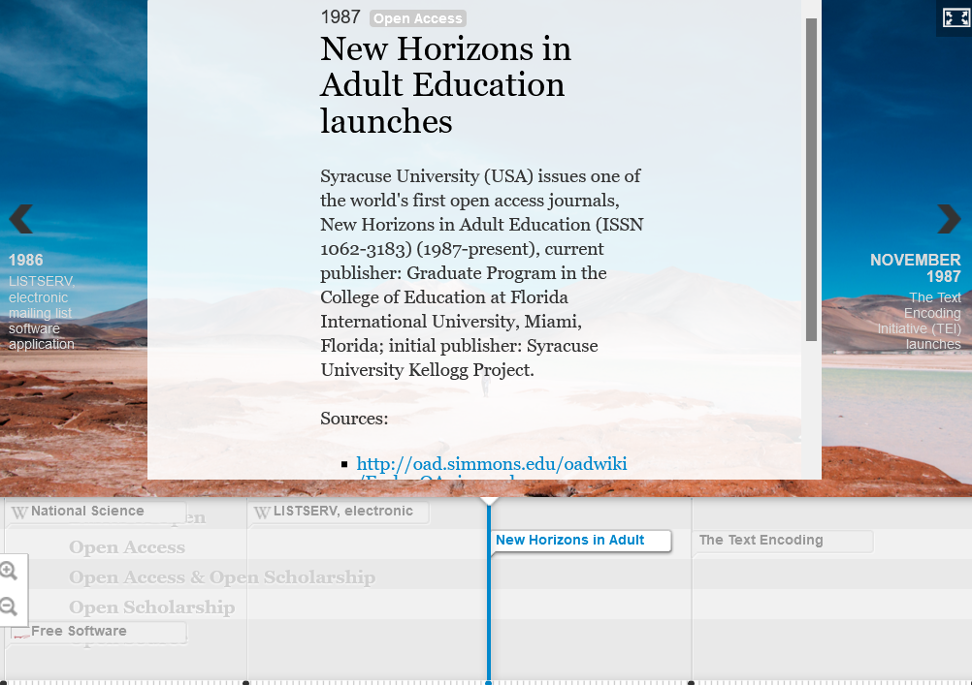
\includegraphics[width=.9\textwidth]{img/abb1.png}
\caption{Abbildung 1: Interaktive Zeitleiste: Geschichte
unterschiedlicher Strömungen zu digitaler Openness: Open Source, Open
Access \& Open Scholarship. Abrufbar unter
\url{https://blog.flavoursofopen.science/timeline-open-source-access-scholarship/}}
\end{figure}

\pagebreak

\hypertarget{fruxfche-scholar-led-experimente-im-digitalen-raum}{%
\section{Frühe scholar-led Experimente im digitalen
Raum}\label{fruxfche-scholar-led-experimente-im-digitalen-raum}}

\begin{quote}
\enquote{Apparently, there are academics, and reputable ones at that,
for whom the cost/benefit of the Mercedes Benz -- the smart cover,
prestigious logo, beautiful paper, and added-value galore -- is less
important than the means of quick and effective conveyance, even if it
be merely a rusty old heap that runs. Academic aspirations are, in many
cases, being modified by the financial realities of the day. I believe
this is leading us to a more differentiated array of publications. I
imagine the Internet full of curiously painted VW beetles and vans, an
engaging mixture of information vehicles. If this speculation becomes
reality, and if our academics and their institutions become aware that
the current style of single-minded high-value publishing can lead to
perishing, then we are headed for some value shifts over time.}
(\href{https://doi.org/10.7202/1064955ar}{Okerson, 1994})
\end{quote}

Für die Geistes- und Sozialwissenschaften spielen frühe, insbesondere
zeitlich \emph{vor} der im ersten Teil angeführten weit verbreiteten
Geschichte von Open Access aufkommenden und mit dem neuen digitalen
Medium experimentierenden scholar-led Publikationsprojekte und
-initiativen eine in der Breite immer noch zu wenig beachtete Rolle. Wie
beispielsweise Moore mit Referenz auf frühe digitale Journal-Initiativen
aufzeigt, existierten schon deutlich vor dem gemeinhin als Start der
Open Access-Bewegung angesehenen frühen 2000er Jahre zahlreiche
scholar-led Initiativen aus den Geistes- und Sozialwissenschaften, die
sich -- auch als Reaktion auf die starke Kommerzialisierung des
Zeitschriftenmarktes in den 1970ern und 1980ern\footnote{\enquote{For
  Okerson, journal publishing was in a \enquote*{dismal} state with over
  71\,\% of journals published by the for-profit sector, which resulted
  in a \enquote*{loss of ownership} of scholarly publishing from the
  academy.} Ann Okerson, 1992, zitiert in
  \href{https://doi.org/10.17613/41h8-j423}{Moore, 2020 {[}2019{]}, S.
  8}.} -- zum Ziel gesetzt hatten, die Produktion und Zirkulation von
Wissenschaftskommunikation im Digitalen selbst zu organisieren und diese
dabei frei öffentlich zugänglich zu gestalten.

Walt Crawford zeigte beispielsweise im angloamerikanischen Kontext schon
2002 auf, dass mehr als 75\,\% der 107 katalogisierten frühen Journals,
die im
\href{http://info.cern.ch/hypertext/DataSources/Journals.html}{Directory
of Electronic Journals, Newsletters and Academic Discussion Lists} (1991
erstmals herausgegeben durch die US-amerikanische Association of
Research Libraries) gelistet wurden, den Geistes- und
Sozialwissenschaften zugeordnet werden konnten (vergleiche.
\href{https://doi.org/10.1087/09531510252848881}{Crawford, 2002}). Und
auch, wenn die eingangs erwähnte Geschichte von Preprints in diesem
Beitrag nur knapp betrachtet werden kann, so ist zudem auffällig, dass
Ann Okerson schon 1994 darauf hinweist, dass neben den STM-Fächern auch
Philosophie und die Philologien als starke Proponenten in der durch die
Association of Research Libraries beforschten frühen Preprint-Kultur
auffielen (vergleiche \href{https://doi.org/10.7202/1064955ar}{Okerson,
1994}).

Hier zeigt sich schon aufgrund der Quantität, wie die \enquote{alte
Tradition}\footnote{Hier mit Bezug auf die Tradition von
  \emph{scholar-led} in den Geistes- und Sozialwissenschaften, in leicht
  abgewandelter Anlehnung an den Eröffnungssatz der Erklärung der
  Budapest Open Access Initiative (BOAI), \enquote{An old tradition and
  a new technology have converged to make possible an unprecedented
  public good.}, siehe
  \url{https://www.budapestopenaccessinitiative.org/read/}.} der auch in
den Geistes- und Sozialwissenschaften durch Wissenschaftler*innen selbst
betriebenen -- also \emph{scholar-led} -- Publikationsorgane durch das
Aufkommen der technischen Möglichkeiten der Digitalität (auch schon vor
dem Internet) neue kreative Outlets entwickelte. Mit Blick auf frühe
Journals der 1990er Jahre schreibt Moore dazu:

\begin{quote}
\enquote{Although nascent or implicit in their practices, these journals
espoused both a commitment to the ‹open access› philosophy (although the
term was not invented yet) and to forms of digital publishing that were
both critical and experimental.}
(\href{http://dx.doi.org/10.17613/gty2-w177}{Moore, 2020})
\end{quote}

Unverkennbar wird auch der durchaus offen utopistische Anspruch vieler
dieser frühen scholar-led Initiativen am Beispiel von Stevan Harnads
\emph{subversive proposal} sehr deutlich:

\begin{quote}
\enquote{The subversion will be complete, because the (esoteric --
no-market) peer-reviewed literature will have taken to the airwaves,
where it always belonged, and those airwaves will be free (to the
benefit of us all) because their true minimal expenses will be covered
the optimal way for the unimpeded flow of esoteric knowledge to all: In
advance.} (\href{https://eprints.soton.ac.uk/362894/}{Harnad, 1995})
\end{quote}

Und in der Tat gehörten Harnad als Gründer von
\href{https://web-archive.southampton.ac.uk/journals.ecs.soton.ac.uk/CogsciDemo/psyc\_hp.html}{Psycoloquy}
oder Jean Claude Guédon, Gründer von
\href{https://www.erudit.org/en/journals/surfaces/}{Surfaces}, zu den
prominenten Vertreter*innen früher im Digitalen agierender geistes- und
sozialwissenschaftlicher Initiativen, die auch bei Moore (2019) als
Beispiele auftauchen. Darüber hinaus lassen sich zahlreiche weitere
Publikationsinitiativen mit geistes- und sozialwissenschaftlichem Bezug
ausfindig machen, die sich zum Ziel gesetzt hatten, aus der Wissenschaft
heraus, also \emph{scholar-led}, Impulse für eine neue Art des
Publizierens und damit der aktiven Gestaltung von Wissenschaft zu
setzen.

Wie im Folgenden ausgeführt wird, setzten sich viele dieser scholar-led
Initiativen aktiv mit der später auch in der Open-Access-Bewegung
verankerten Kernmotivation der freien Verfügbarmachung
wissenschaftlicher Publikationen auseinander. Sie taten dies oftmals mit
einem dezidiert geisteswissenschaftlichen Duktus kritisch-theoretischer
Reflexion über die prozessuale Ausgestaltung desselben. Dies schloss des
Öfteren auch eine radikale\footnote{Im Sinne von \enquote{fundamental},
  die Wurzel betreffend.} Herangehensweise und Grundphilosophie mit ein,
was sich darin widerspiegelte, dass nicht nur Publikationen als Produkte
des wissenschaftlichen Erkenntnisprozesses offen verfügbar gemacht
wurden, sondern im Sinne von
\href{https://library.nuigalway.ie/openscholarship/}{Open Scholarship}
der gesamte Prozess der Entstehung, Kuratierung und Dissemination von
Wissen offen kritisch reflektiert wurde.

\hypertarget{die-vielfalt-geistes--und-sozialwissenschaftlicher-scholar-led-initiativen}{%
\section{Die Vielfalt geistes- und sozialwissenschaftlicher
scholar-led
Initiativen}\label{die-vielfalt-geistes--und-sozialwissenschaftlicher-scholar-led-initiativen}}

Während, wie Janneke Adema schreibt, einzelne \enquote{experiments with
e-books and hypertexts were already taking place in the1960s---if not
earlier} (\href{https://doi.org/10.7551/mitpress/11297.003.0005}{Adema,
2021}), so entwickelte die Verfügbarmachung von wissenschaftlichem
Output im Digitalen erst in den 1970ern etwas mehr Dynamik. Im
internationalen Kontext stehen hier sicherlich selbstorganisierte
Publikationsinitiativen und -communities wie das 1971 gegründete
\href{https://www.gutenberg.org/about/}{Project Gutenberg} oder das
Oxford Archive of Electronic Literature (später
\href{https://ota.bodleian.ox.ac.uk/repository/xmlui/page/about}{Oxford
Text Archive}) in der der Open-Access-Bewegung zugrunde liegenden
Tradition der offenen Verfügbarmachung wissenschaftlicher Publikationen.
Aus dem Feld der Erziehungswissenschaften -- mit Bezug zu Medien und den
emergenten Möglichkeiten des Digitalen -- fallen hier beispielsweise
\href{https://web.archive.org/web/20120701192019/http://education.fiu.edu/newhorizons/journals/vol1n1.txt}{New
Horizons in Adult Education} (1987), das
\href{https://jasonohler.com/OJournal/\#april\%2088}{Online Chronicle of
Distance Education and Communication} (1987/88) oder
\href{https://web.archive.org/web/19970127015651/http://borg.lib.vt.edu/ejournals/JTE/jte-v1n1/contents.jte-v1n1.html}{The
Journal of Technology Education} (1989) durch frühe Aktivitäten im
Digitalen vor dem Launch des World Wide Web auf.

Als Kommunikationskanäle wählten diese frühen scholar-led Initiativen
die schon vor dem Launch des World Wide Web existierenden ftp-, IRC-,
bulletin board system (BBS)- oder Usenet-Protokolle oder auch den
E-Mail-basierten Informationsaustauschs per
\href{https://en.wikipedia.org/wiki/LISTSERV}{Lis}t\href{https://en.wikipedia.org/wiki/LISTSERV}{serv}.
Und auch das parallel zum World Wide Web (WWW) etablierte
gopher-Protokoll diente diesen frühen digitalen scholar-led Communities
als wichtiger Kanal, so wurden beispielsweise das schon genannte
\emph{psycholoquy} oder \emph{Postmodern Culture} (1990) auch über
gopher verfügbar gemacht.\footnote{Andrew Treloar beschreibt in seinem
  1995 veröffentlichten Aufsatz
  \enquote{\href{https://andrew.treloar.net/research/publications/vala96/index.html}{Better
  than Print? Hypermedia Scholarly Publishing and the World Wide Web}}
  die Vorgehensweise bezüglich (A)FTP, Listserv und anderer Protokolle
  im Detail.}

\hypertarget{scholar-led-journal-initiativen-aus-den-kultur--und-medienwissenschaften}{%
\section{Scholar-led Journal-Initiativen aus den Kultur- und
Medienwissenschaften}\label{scholar-led-journal-initiativen-aus-den-kultur--und-medienwissenschaften}}

Die seit den frühen 1990er Jahren stark an Fahrt aufnehmenden
Konvergenz-Bewegungen hin zu digitaler Telekommunikation und die
zunehmende Verbreitung von Heimcomputern und Software, welche wiederum
bald in der Breite den Zugang zum Internet etablierten, erzeugte eine
neue Pluralität an Ausdrucks- und Partizipationsmöglichkeiten -- sowohl
in der Öffentlichkeit als auch in wissenschaftlichen Kreisen.

Für scholar-led Initiativen besonders interessant war und ist der Aspekt
der dezentralisierten und unabhängigen Interaktion, die im Kontrast zur
aus dem Printbereich stark vorherrschenden zentralisierten und
unidirektionalen Kommunikation zumeist über kommerzielle Verlage steht,
da im neuen Medium Internet interaktive Kommunikation direkt passieren
konnte. Hinzu kam der Anreiz der experimentellen Nutzung emergenter
digitaler Technologien, die einem stetig wachsenden Nutzendenkreis
ermöglichten, Ausdrucks- und Publikationsformen zu realisieren, welche
zuvor nur hochprofessionalisierten Spezialist*innen vorbehalten
waren.\footnote{~Hier sind beispielsweise Layouting, digitales
  publishing via CMS (Drupal, WordPress, OJS, et cetera) und
  Print-on-Demand publishing zu nennen. Siehe dazu auch Janneke Adema:
  \href{https://openreflections.wordpress.com/2009/06/23/where-open-philosophy-meets-open-music/}{Where
  Open Philosophy Meets Open Music}, \emph{OPEN REFLECTIONS}, 23.6.2009;
  und Silvio Lorusso:
  \href{https://networkcultures.org/outofink/2011/09/13/interview-with-paul-ashton-co-founder-of-re-press/}{Interview
  with Paul Ashton, co-founder of re.press}, \emph{Out of Ink \textbar{}
  Future of the Publishing Industry}, 13.9.2011.} Des Weiteren spielt
sicherlich der Faktor des Kostendrucks, der sich insbesondere in der
sogenannten Zeitschriftenkrise der 1970er und 1980er manifestierte, eine
immer größere Rolle und diente als Motivation für viele scholar-led
Initiativen, selbstorganisiert Alternativen zur bestehenden
Publikationslandschaft zu entwickeln -- und diese wurden im digitalen
Raum plötzlich möglich.

Speziell mit Blick auf die Kultur- und Medienwissenschaft sind hier
einige regionale Beispiele wie das britische
\href{https://www.radicalphilosophy.com/editorial/founding-statement-frontispiece}{Radical
Philosophy} (1972--), das skandinavische
\href{https://www.nordicom.gu.se/en/publications/nordicom-review/nordicom-review-11996}{Nordicom
Review} (1980--,
\href{https://www.nordicom.gu.se/en/publications/nordicom-review/nordicom-review-11996}{Open
Access}\footnote{Auch wenn die Bezeichnung \enquote{Open Access} zu dem
  Zeitpunkt noch gar nicht existierte.}
\href{https://www.nordicom.gu.se/en/publications/nordicom-review/nordicom-review-11996}{seit
1996}), das 1985 gestartete dänische
\href{https://tidsskrift.dk/mediekultur/}{MedieKultur: Journal of media
and communication research}, die gemeinsam mit den Anfängen des WWW
gestarteten
\href{https://archive.org/details/DGRD_01_zip\%20https://archive.org/search.php?query=creator\%3A\%22Dave\%20Taylor\%22\%20Digital\%20Games\%20Review}{Digital
Games Review}, das kanadische
\href{http://ejcojs.cios.org/index.php/ejc}{Electronic Journal of
Communication / La Revue Electronic de Communication} (alle 1990), oder
auch die US-amerikanischen
\href{http://pmc.iath.virginia.edu/text-only/issue.990/contents.990.html}{Postmodern
Culture} (1990) und
\href{https://web.archive.org/web/20000305174913/http://rachel.albany.edu/~ejournal/v1n1/v1n1.html}{eJournal}
(1991) relevant.\footnote{Hier muss der Vollständigkeit halber ergänzt
  werden, dass weitere frühe Beispiele aus der deutschsprachigen
  Medienwissenschaft wie beispielsweise \emph{MEDIENwissenschaft
  Rezensionen \textbar{} Reviews} (1984), \emph{AugenBlick. Konstanzer
  Hefte zur Medienwissenschaft} (1985) oder \emph{montage AV} (1992) für
  diese Übersicht initial auch in Betracht gezogen wurden -- da sie in
  Zusammenarbeit mit dem Schüren Verlag herausgegeben werden, fallen sie
  jedoch nicht in die engere Auswahl, da die externalisierte
  verlegerische Tätigkeit nicht unter die Definition selbstorganisierter
  scholar-led-Initiativen (siehe definitorischer Teil dieses Beitrags)
  fällt.}

All diese Beispiele stehen dafür, wie scholar-led Communities aus den
Geistes- und Sozialwissenschaften sich schon früh und teilweise deutlich
vor der Geburtsstunde des WWW emergent mit offener digitaler
Kommunikation sowohl als Forschungsgegenstand, als auch als einen die
eigene Wissenschaftspraxis reflektierenden Kommunikationskanal
auseinandersetzen. Im Laufe der 1990er Jahre formten sich sowohl
internationale als auch deutschsprachige scholar-led Communities
beispielsweise über das 1994 initiierte
\href{https://www.h-net.org/lists/}{H-Net}. Zudem kamen zahlreiche frühe
für die Kultur- und Medienwissenschaft relevante Journal-Initiativen wie
\href{https://doi.org/10.5210/fm.v1i1.464}{First Monday} (1996),
\href{https://web.archive.org/web/20130305050839/http://www.film-philosophy.com/index.php/f-p/issue/view/3}{Film-Philosophy}
(1997),
\href{https://www.medienobservationen.de/redaktion/}{Medienobservationen}
(1997), die
\href{https://web.archive.org/web/19990117055559/http://www.rz.uni-frankfurt.de/FB/fb09/muwi/FZMw.html}{Frankfurter
Zeitschrift für Musikwissenschaft} (1997),
\href{https://journal.media-culture.org.au/index.php/mcjournal/issue/view/new}{M/C
Journal} (1998), das \href{https://www.tmgonline.nl/about/}{TMG Journal
for Media History} (1998), \href{https://culturemachine.net/}{Culture
Machine} (1999),
\href{https://nachdemfilm.de/issues/no-1-das-kino-bebt}{Nach dem Film}
(1999) und
\href{https://www.transformationsjournal.org/}{Transformations} (2000)
hinzu.

Mit den um die Jahrtausendwende in der Breite Einzug haltenden digitalen
Innovationen wie Zugang zum WWW, instant messaging, WebLogs/Blogs,
Wikis, sozialen Netzwerken, et cetera wuchs auch der Kreis der
potentiell an wissenschaftlicher Kommunikation Partizipierenden
exponentiell -- und damit auch die Vielfalt an scholar-led
Publikationsinitiativen. So startete das neue Jahrtausend mit weiteren
scholar-led Journals wie
\href{https://www.imageandnarrative.be/inarchive/index.htm}{Image
{[}\&{]} Narrative} (2000) und
\href{https://journals.sub.uni-hamburg.de/hup2/kommges/backlist}{kommunkation@gesellschaft}
(2000), und 2001 folgten
\href{http://rhizomes.net/files/issues.html}{Rhizomes: Cultural Studies
in Emerging Knowledge},
\href{http://www.ephemerajournal.org/what-ephemera}{ephemera: theory \&
politics in organization},
\href{https://www.kunsttexte.de}{kunsttexte.de}, das Schweizer
\href{https://www.hope.uzh.ch/scoms}{Studies in Communication Sciences}
sowie das an der Universität Siegen herausgegebene
\href{https://www.universi.uni-siegen.de/katalog/zeitschriften/navigationen/}{Navigationen
- Zeitschrift für Medien- und Kulturwissenschaften}.

2003 begannen \href{https://fibreculturejournal.org/}{Fibreculture
Journal} sowie
\href{https://www.triple-c.at/index.php/tripleC/about}{tripleC
Communication, Capitalism \& Critique}, 2004 die
\href{https://www.westminsterpapers.org/}{Westminster Papers in
Communication and Culture}, und 2005 folgten
\href{https://www.flusserstudies.net/archive}{Flusser Studies:
Multilingual Journal for Cultural and Media Theory},
\href{http://vectors.usc.edu/archive/}{Vectors},
\href{https://americanaejournal.hu/about}{AMERICANA}, sowie das an der
Universität Tübingen gestartete
\href{http://www.gib.uni-tuebingen.de/image}{IMAGE}.

In den späteren 2000er Jahren betraten
\href{http://www.tripodos.com/index.php/Facultat_Comunicacio_Blanquerna/about}{Tripodos}
(2006),
\href{https://mediacommons.org/imr/archives?sort_bef_combine_date=created+ASC}{In
Media Res} (2007),
\href{https://web.archive.org/web/20210122132539/http:/www.darkmatter101.org/site/about/}{darkmatter} (2007), das \href{https://ijoc.org/index.php/ijoc/about}{International
Journal of Communication} (2007) sowie die
\href{https://journals.qucosa.de/kbzf}{Kieler Beiträge zur
Filmmusikforschung} (2008),
\href{https://soundstudiesblog.com/}{sounding out!} (2009),
\href{https://dj.dancecult.net/index.php/dancecult/issue/view/39}{Dancecult}
(2009) und \href{https://cultureunbound.ep.liu.se/}{Culture Unbound}
(2009) die Bühne. Die frühen 2010er Jahre sahen eine neue Welle von
scholar-led Journals; so starteten
\href{http://www.alphavillejournal.com/}{Alphaville} (2010),
\href{https://www.uni-weimar.de/rabbiteye/}{RabbitEye} (2010), sowie
\href{https://limn.it/issues/prototyping-prototyping/}{Limn} (2010/11),
und
\href{https://cstonline.net/cst-online-relaunch-by-kim-akass/}{CSTOnline}
(2011), das offene scholar-led Companion-Blog des Journals
\emph{Critical Studies in Television}, feierte 2011 seinen Relaunch.

Des weiteren kamen \href{http://openthresholds.org/}{thresholds} (2011),
\href{https://www.paidia.de/}{Paidia -- Zeitschrift für
Computerspielforschung} (2011), das
\href{https://web.archive.org/web/20120510164302/http://peerproduction.net/issues/issue-0/}{Journal
of Peer Production} (2011, nicht mehr aktiv),
\href{https://reframe.sussex.ac.uk/sequence1/}{SEQUENCE} (2012),
\href{https://viewjournal.eu/about/}{VIEW Journal of European Television
History and Culture} (2012) \href{https://www.sdvigpress.org}{sdvig
press} (2012), sowie vier Journals, die 2013 begannen, hinzu:
\href{https://zapruderworld.org/journal/past-volumes/}{ZapruderWorld},
\href{https://zeitschrift-suburban.de/sys/index.php/suburban/}{sub\textbackslash urban.
zeitschrift für kritische stadtforschung},
\href{https://feralfeminisms.com}{feral feminisms}, sowie die eigentlich
schon 1987 gestartete
\href{https://www.fkw-journal.de/index.php/fkw/about}{FKW // Zeitschrift
für Geschlechterforschung und visuelle Kultur} hinzu, welche 2013 ihr
Archiv offen verfügbar machte und seitdem auch Open Access publiziert.
Das am Centre for Digital Cultures (CDC) der Leuphana University
Lüneburg angesiedelte \href{https://spheres-journal.org/about/}{spheres:
Journal for Digital Cultures} startete 2014, und
\href{https://www.sahjournal.com/site/about/}{Studies in Arts and
Humanities} sowie \href{http://digicults.org/}{Digital Culture \&
Society} kamen 2015 hinzu.

2016 entschied das seit 1988 jährlich organisierte
\href{http://kolloquium.ffk-journal.de/fundstuecke/}{Film- und
Fernsehwissenschafliche Kolloquium} (seit 2022 \emph{Film- und
Medienwissenschaftliches Kolloquium}), ein eigenes Journal mit jährlich
wandernden Herausgebenden-Teams ins Leben zu rufen, welches kurz danach
in Kooperation mit dem scholar-led Verlag AVINUS unter dem Namen
\href{http://www.ffk-journal.de/}{ffk Journal} realisiert wurde. Im
gleichen Jahr wurde das Archiv von
\href{https://www.radicalphilosophyarchive.com/this-archive/}{Radical
Philosophy} offen verfügbar gemacht, und
\href{https://www.mediaesthetics.org/index.php/mae/issue/view/5}{medi\emph{a}esthetics
-- Journal of Poetics of Audiovisual Images},
\href{https://www.mutualimages-journal.org/}{Mutual Images} sowie
\href{https://www.on-culture.org/journal/}{On\_Culture} nahmen die
Arbeit auf. 2017 erschienen sowohl
\href{https://opengenderjournal.de/}{Open Gender Journal} als auch
\href{https://journalcontent.mediatheoryjournal.org/index.php/mt/issue/view/1}{Media
Theory} zum ersten Mal, während 2019
\href{https://21-inquiries.eu/en/about-the-journal/}{21: Inquiries} und
2021
\href{https://www.gamescoop.uni-siegen.de/spielformen/index.php/journal}{Spielformen}
sowie \href{https://hms.mediastudies.press/}{History of Media Studies}
den Kreis der scholar-led Journals weiter vergrößerten.

Wie in all diesen Beispielen deutlich sichtbar wird, sollte Ann Okerson
mit ihrer oben zitierten Einschätzung zumindest für einen Teil der
Geistes- und Sozialwissenschaften Recht behalten: In so gut wie allen
der hier aufgeführten wissenschaftlichen Communities ist deutlich der
Wunsch nach Etablierung von selbstorganisiert gesteuerten und offenen
Kommunikationsinfrastrukturen zu erkennen.

\hypertarget{scholar-led-buchverlage-in-den-geistes--und-sozialwissenschaften}{%
\section{Scholar-led Buchverlage in den Geistes- und
Sozialwissenschaften}\label{scholar-led-buchverlage-in-den-geistes--und-sozialwissenschaften}}

\begin{quote}
\enquote{{[}M{]}ight it not be helpful to think of open access
\emph{less} as a project and model to be implemented, and \emph{more} as
a process of continuous struggle and critical Resistance?}
(\href{https://doi.org/10.3898/NewF.78.07.2013}{Adema \& Hall, 2013})
\end{quote}

\begin{quote}
\enquote{{[}I{]}f we are theorists, if we are radical, critical
theorists, then our critique should aim at a transformation of the
actual systems within which we work.}
(\href{https://repository.jisc.ac.uk/6652/}{Joy, 2017})
\end{quote}

Es muss konstatiert werden, dass die Anzahl der scholar-led Buchverlage
deutlich geringer ausfällt, als dies bei den im vorherigen Abschnitt
gelisteten Journal Communities der Fall ist. Dies ist sicherlich darauf
zurückzuführen, dass sich der zu investierende Aufwand in der Produktion
und Dissemination von Buchpublikationen deutlich komplexer und das
dadurch nötige Commitment zum Betrieb eines scholar-led Buchverlags umso
substantieller gestaltet.

Umso relevanter scheint daher die Signifikanz der Entwicklungen in
diesem Bereich, denn auch hier hat sich eine Vielzahl von Initiativen
herausgebildet, die aus der Wissenschaftscommunity heraus organisiert,
oft mit klarem Fachbezug, unabhängig und nicht profitorientiert
wissenschaftliche Buchpublikationen verlegen und dabei oftmals die
Grenzen dessen, was ein Buch im digitalen Raum ausmacht, in seiner
konzeptuellen Form durch experimentelle Ansätze immer wieder neu
definieren.

So betrat beispielsweise David Kolb schon 1994 mit der
Hypertext-Buchpublikation
\href{http://www.eastgate.com/catalog/Socrates.html}{Socrates in the
Labyrinth: Hypertext, Argument, Philosophy} -- wenn auch mittels
kommerzieller Plattformen -- früh neues Terrain damit, eine
philosophische Abhandlung mit den Möglichkeiten des Hypertext
zusammenzubringen.\footnote{Siehe dazu auch die
  \href{https://scalar.usc.edu/works/rebooting-electronic-literature/photos-of-david-kolbs-socrates-in-the-labyrinth}{Abbildungen
  in Dene Grigars Rebooting Electronic Literature}, 2018.} Kurz danach,
1995, wagte sich William J. Mitchell experimentell daran, mit
\href{https://mitpress.mit.edu/9780262631761/city-of-bits/}{City of
Bits} (kommerziell über MIT Press publiziert) die Möglichkeiten des
Digitalen im Kontext urbaner Architektur in hybrider Buchform zu
erforschen.\footnote{Siehe dazu auch William Mitchells die eigene Praxis
  reflektierenden Aufsatz
  \href{http://mitpress2.mit.edu/e-books/City_of_Bits/Text_Unbound/text_unbound.html}{Homer
  to Home-Page: Designing Digital Books}, Februar 1996.} Und Eric Eldred
begann im gleichen Jahr
\href{https://firstmonday.org/ojs/index.php/fm/article/view/1059/979}{mit
Eldritch Press, ähnlich wie zuvor schon Project Gutenberg, gemeinfreie
Bücher} der Öffentlichkeit online zur Verfügung zu stellen. Eldritch
Press sah sich innerhalb weniger Jahre einem vielbeachteten und
\href{https://archive.nytimes.com/www.nytimes.com/library/tech/99/01/cyber/cyberlaw/15law.html}{wegweisenden
Urheberrechts-Prozess} ausgesetzt, dessen Ausgang eine der
Gemeinnützigkeit zugewandte Interpretation von Fair Use in den USA
deutlich erschwerte und unter anderem 2001 zur Gründung von Creative
Commons und deren Bereitstellung eines einheitlichen
Copyleft-Lizenz-Toolkits\footnote{Als Anekdote scheint mir hier
  bemerkenswert, dass Eric Eldred eine
  \href{https://web.archive.org/web/20030115160926/http://www.creativecommons.org/licenses/eldred-pd}{eigene
  Public-Domain-Lizenz für Eldritch Press unter dem Label
  \enquote{Eldred PD} gewidmet wurde}.} führte.

Als ein deutschsprachiger, sich mit Aspekten von Open Access
beschäftigender scholar-led Pionier in den Kultur- und
Medienwissenschaften kann sicherlich der 1992 gegründete
\href{https://produkte.avinus.de/avinus/ueber-den-verlag}{AVINUS Verlag}
gelten, welcher seit 2004 als Zweckbetrieb dem
\href{https://verein.avinus.org/}{AVINUS e.V.} zugeordnet ist. Auch wenn
AVINUS nicht primär als Open-Access-Verlag zu verorten ist -- den
Großteil seiner Publikationen vertreibt der Verlag klassisch über
kommerzielle Kanäle, um entstehende Produktionskosten zu decken -- so
ist doch herauszustellen, dass der Verlag das
\href{http://repositorium.medienkulturforschung.de/}{Repositorium
Medienkulturforschung} (RMKF) im Sinne einer dezidierten
Open-Access-Plattform aufgebaut hat. Das RMKF wiederum wurde jüngst in
den Bestand des seit 2017 am Institut für Medienwissenschaft der
Universität Marburg betriebenen Fachrepositoriums
\href{https://mediarep.org/}{media/rep/} überführt. Zudem sichert der
AVINUS Verlag als rechtlich verantwortliche Entität den Betrieb des
\href{http://ffk-journal.de/}{ffk journal} und trägt über beide Kanäle
aktiv dazu bei, wissenschaftliche Publikationen dieser Communities frei
öffentlich zugänglich zu machen.

Weitere scholar-led Verlage, die sich der grundsätzlichen Idee von Open
Access in einem oftmals als radikal\footnote{Wie schon zuvor im Text ist
  \enquote*{radikal}› hier in der Konnotation von
  \enquote*{grundsätzlich}, \enquote*{die Wurzel betreffend} zu
  verstehen.} bezeichneten Verständnis verpflichtet sehen, entstanden in
den frühen 2000er Jahren oftmals aus schon bestehenden scholar-led
Communities und/oder um einzelne zentrale scholar-led Akteur*innen
herum, die die emergenten Möglichkeiten des digitalen Raums aktiv
nutzten und für sich adaptierten. Unter anderem ermöglicht durch das
Aufkommen erster Print-On-Demand-Dienste sowie frei nutzbarer
Open-Source-Systeme,\footnote{Siehe beispielsweise Joe Deville:
  \href{https://www.matteringpress.org/blog/open-access-publishing-and-the-future-of-the-university}{Open
  Access Publishing and the Future of the University} oder Janneke Adema
  und Samuel A. Moore:
  \href{https://doi.org/10.1629/uksg.399}{Collectivity and
  Collaboration: Imagining New Forms of Communality to Create Resilience
  in Scholar-Led Publishing}.} die scholar-led Verlagen ein schlankes
Geschäftsmodell ermöglichten, begannen beispielsweise
\href{http://mayflybooks.org/?page_id=2}{MayFly Books} (2005 aus dem
\emph{ephemera} Journal-Kollektiv heraus entwickelt),
\href{http://www.openhumanitiespress.org/about/community/}{Open
Humanities Press} (2006 aus der \emph{Culture Machine}-Community heraus
geformt), \href{https://re-press.org/}{re.press} (2006), und
\href{https://www.openbookpublishers.com/section/14/1}{Open Book
Publishers} (2008) damit, wissenschaftliche Monographien, Sammelwerke
und alles, was sich unter dem Format der in den Geistes- und
Sozialwissenschaften so wichtigen Langform subsumieren lässt, teilweise
mit klarem fachspezifischem Fokus, teilweise auch in einem breiteren
Spektrum anzubieten.

Seit 2010 kamen dann
\href{https://ebooks.americanaejournal.hu/about/}{AMERICANA ebooks},
\href{https://www.editionscienceetbiencommun.org/en/}{Éditions science
et bien commun},
\href{https://punctumbooks.com/about/vision-statement/}{punctum books},
\href{https://www.matteringpress.org/about}{Mattering Press},
\href{https://www.africanminds.co.za/}{African Minds} sowie
\href{https://counterpress.org.uk/about/}{Counterpress} und
\href{https://www.theoperatingsystem.org/}{The Operating System} hinzu.
2014 starteten sowohl
\href{https://web.archive.org/web/20160113000302/http://www.rovingeyepress.com/}{Roving
Eye Press}, \href{https://langsci-press.org/about}{Language Science
Press}, als auch \href{https://meson.press/about/}{meson press}, welches
als Spin-off aus dem Hybrid Publishing Lab des Centre for Digital
Cultures (CDC) der Leuphana Universität in Lüneburg ausgegründet
wurde.\footnote{Siehe hierzu auch das empfehlenswerte
  \href{https://jussiparikka.net/2014/07/11/a-mini-interview-mercedes-bunz-explains-meson-press/}{Interview
  mit Mercedes Bunz}, Mitbegründerin von meson press, geführt von Jussi
  Parikka.} 2016 rief Sarah-Mai Dang, Mitbegründerin des
Open-Media-Studies-Blogs, den scholar-led Verlag
\href{https://www.oabooks.de/verlag/}{oa books} ins Leben. 2017 formte
sich \href{https://hcommons.org/members/pop/}{Post Office Press} als
experimentelles Projekt am Centre for Postdigital Cultures der Coventry
University. 2018 publizierte
\href{http://electric.press/about.html}{electric.press} (firmiert auch
unter dem Namen Hyperrhiz Electric) ihr
\href{http://electric.press/books/middleshore.html}{erstes
Langform}-Experiment. 2019 startete Jeff Pooley
\href{https://www.mediastudies.press/}{mediastudies.press} und im
gleichen Jahr begann auch
\href{https://flugschriften.com}{FlugSchriften} mit der Arbeit.

\hypertarget{positionierungen-von-scholar-led-initiativen}{%
\section{Positionierungen von scholar-led
Initiativen}\label{positionierungen-von-scholar-led-initiativen}}

Wie eingangs schon erwähnt, positionieren sich viele scholar-led
Initiativen deutlich als abseits des kommerziell betriebenen
Publikationswesens bestehend. Diese Positionierung als Alternative
beziehungsweise Gegenentwurf zu kommerziellen Verlagen wird
beispielsweise bei Counterpress sehr deutlich:

\begin{quote}
\enquote{We set up COUNTERPRESS in 2013 as a \enquote*{counter} to the
privatizing and excessive profiteering of academic knowledge and to do
away with unfair access restrictions to learning materials in a world of
uneven globalization.}
(\href{https://counterpress.org.uk/about/}{COUNTERPRESS -
\enquote*{About}}).
\end{quote}

Ähnliche Positionierungen, die die Frustration gegenüber sowie eine
grundsätzliche Kritik am bestehenden Publikationssystem und der daraus
motivierten Suche nach Alternativen wiederspiegeln, lassen sich bei
zahlreichen scholar-led Initiativen, beispielsweise bei
\href{https://mayflybooks.org/about/}{Mayfly Books},
\href{https://punctumbooks.com/about/vision-statement/}{punctum books},
und
\href{https://blogs.openbookpublishers.com/ten-years-of-obp-an-interview-with-alessandra-tosi-and-rupert-gatti/}{Open
Book Publishers}, aber auch bei vielen der im zweiten Teil genannten
Journal-Initiativen wiederfinden. Eileen Joy von punctum books stellt
heraus:

\begin{quote}
\enquote{{[}Our aim is to take{]} back from commercial publishers the
full reins of the means of production of academic publishing and
reinventing the academic press as a critical arm of both the research
and teaching mission of the University.} (Joy, 2020)
\end{quote}

Wie unter anderem bei
\href{https://twitter.com/hardyjuls/status/1314347568185462786}{mattering
press} und Open Humanities Press deutlich wird, haben viele scholar-led
Initiativen zum Ziel, alternative, unabhängige Räume zu schaffen, in
denen dem sonst weithin bestehenden Mangel an aktivem Engagement und
Experimentierfreudigkeit mit Theorie und Praxis des Publikationswesens
in den Geistes- und Sozialwissenschaften aktiv begegnet werden kann.
Hierzu wird beispielsweise im Interview mit Kathleen Fitzpatrick
deutlich, dass sich scholar-led Initiativen um einiges flexibler in der
Realisation experimenteller Ansätze\footnote{Für eine Übersicht
  aktueller experimenteller Buchpublikationspraktiken, dazu geeigneter
  Open-Source-Plattformen sowie Beispielpublikationen siehe
  beispielsweise der im COPIM-Projekt entstandene Scoping Report
  \href{https://doi.org/10.21428/785a6451.1792b84f}{Books Contain
  Multitudes: Exploring Experimental Publishing (2022 update)} sowie das
  jüngst veröffentlichte
  \href{https://compendium.copim.ac.uk}{Experimental Publishing
  Compendium}.} sehen, als dies etablierte Universitätsverlage oder gar
große kommerzielle Anbieter sein können:

\begin{quote}
\enquote{Fitzpatrick said that when she set up Media Commons Press
university presses were not technologically equipped to support
experimental scholarship; they would not be able \enquote*{to do that
kind of experimentation without a whole lot of study, a whole lot of
preparation, and a whole lot of practical concerns that, as an
individual, I simply didn't have at that time}.}
(\href{https://repository.jisc.ac.uk/6666/1/Changing-publishing-ecologies-report.pdf}{Fitzpatrick,
2017})
\end{quote}

Wie Janneke Adema und Graham Stone (2017) und Judith Fathallah (2023)
anhand zahlreicher Interviews mit scholar-led Verlagen herausgearbeitet
haben, folgen viele scholar-led Initiativen einem auf Gemeinnützigkeit
und nicht auf Profitmaximierung ausgelegten Betriebsmodell. So manche
Vertreter*in versteht sich als Teil eines heterogenen, pluralistischen
und auf Nichtrivalität\footnote{Siehe zu \enquote{non-rivalrous goods}
  im Open-Access-Kontext beispielsweise
  \href{https://knowledgeunbound.mitpress.mit.edu/pub/cjktrtqe/release/1}{Suber
  2016} oder \href{https://doi.org/10.5210/fm.v23i2.8161}{Olleros 2018}.}
basierenden alternativen Ökosystems der Wissensallmende beziehungsweise
\emph{Commons}.\footnote{Für Näheres zum Thema Wissensallmende
  beziehungsweise \emph{Knowledge Commons} siehe beispielsweise das von
  David Bollier geführte Podcast-Interview mit Sam Moore
  \enquote{\href{http://www.bollier.org/blog/radical-open-access-collective-building-better-knowledge-commons,}{The
  Radical Open Access Collective: Building Better Knowledge Commons}},
  oder weiterführend \href{http://doi.org/10.1629/uksg.399}{Adema \&
  Moore 2018} sowie \href{https://doi.org/10.17613/st5m-cx33}{Moore
  2019}.} Dieses ist nicht auf Wettbewerb ausgerichtet und setzt auf
horizontale Kollaboration auf Augenhöhe, zu welcher Adema und Stone
konstatieren:

\begin{quote}
\enquote{It becomes clear from the interviews that this principle of
sharing and of not being in competition with others is quite common
among the presses we interviewed, and they often share expertise and
even tend to publish together. {[}...{]} This sharing of information and
advice is part of an ongoing ethos of collaboration and gifting, often
in stark opposition to the closed-off and proprietary business and
publishing models of commercial publishers.}
(\href{https://repository.jisc.ac.uk/6666/}{Adema \& Stone, 2017})
\end{quote}

Dieser der Arbeitsweise vieler scholar-led Initiativen zugrundeliegende
rege Austausch, der auch die die eigene Arbeit limitierenden
Herausforderungen nicht ausspart,\footnote{Vergleiche beispielsweise
  Deville et al. \href{https://doi.org/10.18352/lq.10277}{2019}, oder
  für den DACH-Kontext der
  \href{https://doi.org/10.18452/21418}{LIBREAS-Beitrag von Kathrin
  Ganz, Marcel Wrzesinski und Markus Rauchecker}.} führt auch dazu, dass
sich zahlreiche scholar-led Netzwerke bilden konnten, auf die ich im
Folgenden eingehen möchte.

\hypertarget{scholar-led-kollaborationen-infrastrukturen-netzwerke-kollektive}{%
\section{scholar-led Kollaborationen: Infrastrukturen, Netzwerke
\&
Kollektive}\label{scholar-led-kollaborationen-infrastrukturen-netzwerke-kollektive}}

Auch wenn diese im westlich geprägten Diskurs um Open Access oftmals
schnell vergessen werden, so sind scholar-led Initiativen in einigen
Regionen der Welt weit verbreitet. So existiert beispielsweise in
Lateinamerika schon seit mehr als 40 Jahren eine Tradition des
scholar-led publishing. Netzwerke wie das 1967 gegründete
\href{https://www.clacso.org/en/what-is-clacso/}{Consejo Latinoamericano
de Ciencias Sociales} (CLACSO), das unter der Schirmherrschaft von
CLACSO 2006 gegründete \href{https://www.redalyc.org/}{Redalyc},
\href{http://amelica.org/index.php/en/about/}{AmeliCA}, oder
\href{https://scielo.org/}{ScIELO} zählen zu den großen
lateinamerikanischen Initiativen, die quer über die Geistes- und
Sozialwissenschaften Wissenschaftskommunikation nach nicht
profitorientierten Modellen realisieren. Zudem ist
\href{https://ariadnaediciones.cl/}{Ariadna Ediciones} zu nennen, das
als scholar-led Initiative schon seit 2004 sowohl Bücher, Journals, als
auch einzelne Artikel publiziert.

In Frankreich wurde 1999
\href{https://www.openedition.org/19220}{revues.org} als zentrales
Publikationsforum für die Geistes- und Sozialwissenschaften aus der
Taufe gehoben. Die auf der Open-Source-Software
\href{https://www.lodel.org/666}{Lodel} basierende und
\href{https://oep.hypotheses.org/1909}{2017 in OpenEdition umbenannte}
Plattform bietet zahlreichen Publikationsinitiativen aus dem
französischen und europäischen Raum eine zentrale technische Basis zum
Betrieb von digitalen Journalen. Ähnliche Plattformen mit nationaler
Reichweite wurden seitdem auch in Nordamerika
(\href{https://www.erudit.org/en/}{érudit}, schon 1998), Finnland
(\href{https://journal.fi/}{journals.fi}), den Niederlanden
(\href{https://openjournals.nl/}{openjournals.nl}) und Dänemark
(\href{https://tidsskrift.dk/}{tidsskrift.dk}) etabliert. Allerdings
muss angemerkt werden, dass diese Initiativen, obwohl unbestritten
wichtig als Basisinfrastrukturen für nichtkommerziellen Open Access,
nicht unter die engere Lesart von scholar-led publishing fallen, da sie
primär durch Infrastrukturanbieter-Konsortien betrieben werden.

Während revues.org und ähnliche Initiativen als zentralisierte Angebote
konzipiert sind, ist eine weitere scholar-led Infrastrukturentwicklung
genau umgekehrt auf Dezentralität ausgelegt. 1998 startete John
Willinsky in Kanada das \href{https://pkp.sfu.ca/about/history/}{Public
Knowledge Project} (PKP) im Department of Language and Literacy
Education an der erziehungswissenschaftlichen Fakultät der University of
British Columbia, um not-for-profit Open-Source-Software für offenes,
digitales Publishing zu entwickeln. Drei Jahre später, 2001, erblickte
das \href{https://pkp.sfu.ca/ojs/}{Open Journal Systems} (OJS) des PKP
die Welt -- und veränderte damit die Publikationslandschaft nachhaltig:
Der Vorteil von OJS gegenüber zentralen Angeboten wie revues.org besteht
darin, dass jede noch so kleine Community\footnote{Oder eben auch
  föderierte Meta-Communities beispielsweise auf nationaler Ebene, wie
  im Fall von \href{https://journal.fi/}{journal.fi}.} ihre eigene
OJS-Instanz betreiben und nach den eigenen Bedürfnissen modifizieren
kann, vorausgesetzt sie verfügt über die technischen Grundkenntnisse,
entsprechende Anpassungen am selbstgehosteten Grundsystem vorzunehmen.
Gemeinsam mit dem PKP verkörpert Willinsky, wie Gary Hall schreibt, eine
Vision von \enquote{open access as helping, in a democratic manner, to
produce a form of global information commons and revitalized public
sphere.} (2008, S. 196)

In Großbritannien wurden 2003
\href{https://culturemachine.net/the-e-issue/cultural-studies-e-archive-project/}{Überlegungen
zu einem \enquote{ArXiV für die Cultural Studies}} angeschoben, welches
im Kontext des Journals \emph{CultureMachine} unter dem Titel
\href{https://web.archive.org/web/20080529134559/http://scm-rime.tees.ac.uk/VLE/DOMAIN/CSeArch/TABS/About.asp}{Cultural
Studies e-archive} (CSeARCH) ins Leben gerufen wurde, heute aber nicht
mehr aktiv betrieben wird.

An der Hogeschool van Amsterdam wurde 2004 das
\href{https://networkcultures.org/about/}{Institute of Network Cultures}
(INC) gegründet, das seitdem auch als (institutioneller)
\href{https://networkcultures.org/publications/}{Publisher auftritt}. Im
gleichen Jahr nahm in den USA die
\href{https://blogs.cofc.edu/babelworkinggroup/2005/07/}{BABEL working
group} die Arbeit auf. Zeitgleich begann das
\href{https://eliterature.org/2005/03/the-institute-for-the-future-of-the-book/}{Institute
for the Future of the Book} mit der Arbeit -- alle drei Initiativen
waren seitdem an zahlreichen für die Geistes- und Sozialwissenschaften
relevanten Kollaborationen beteiligt. Eine davon ist das durch Avi Santo
und Kathleen Fitzpatrick 2006 gestartete und bis heute insbesondere für
die Medienwissenschaften relevante
\href{https://mediacommons.org/about}{MediaCommons}-Projekt und
-Netzwerk. Zu einigen der in MediaCommons gestarteten Spin-Offs zählen
\href{https://mediacommons.org/imr/}{In Media Res} sowie
\href{https://mcpress.media-commons.org/}{MediaCommons Press}.

Ebenfalls 2004 startete
\href{https://www.flowjournal.org/test-page/}{Flow}, ein
\enquote{critical forum on media and culture published by the Department
of Radio-Television-Film at the University of Texas at Austin}. Ein paar
Jahre später, 2009, wurde unter Verwendung der
Open-Source-Bloggingplattform WordPress an der City University of New
York (CUNY) damit begonnen, das CUNY Academic Commons-Netzwerk zu
etablieren, welches 2011 als \href{https://commonsinabox.org/}{Commons
in a Box} der breiten Öffentlichkeit zur selbstorganisierten
Weiternutzung bereitgestellt wurde und seitdem auch zahlreichen anderen
Communities wie beispielsweise \href{https://hcommons.org/}{Humanities
Commons} als offene technische Plattform dient.\footnote{Siehe dazu auch
  Audrey Watters:
  \href{https://www.insidehighered.com/blogs/hack-higher-education/commons-box-importance-open-academic-networks}{\enquote{Commons
  in a Box} \& the Importance of Open Academic Networks}, \emph{Inside
  Higher Ed}, 28.11.2011.} Ebenso im Jahr 2011 nahm
\href{https://lantern.mediahist.org/}{Lantern}, die Suchplattform der
\href{http://mediahistoryproject.org}{Media History Digital Library}
(MHDL), den Betrieb auf.\footnote{Zur \emph{working theory} des
  Gründungstrios siehe Eric Hoyt, Wendy Hagenmaier, Carl Hagenmaier:
  \href{https://dx.doi.org/10.1349/PS1.1938-6060.A.430}{Media + History
  + Digital + Library: An Experiment in Synthesis}, in: \emph{Journal of
  E-Media Studies}, Bd. 3, Nr. 1, 2013.} MHDL wiederum ist eine am
Wisconsin Center for Film and Theater Research beheimatete scholar-led
Initiative, die historische Bücher und Periodika aus dem Film-, Fernseh-
und Rundfunkbereich im Sinne von public domain offen zugänglich stellt.

2012 wurde am Centre for Digital Cultures (CDC) der Leuphana University
Lüneburg das
\href{https://www.leuphana.de/en/research-centers/cdc/labs-projects/finished-projects/hybrid-publishing-lab.html}{Hybrid
Publishing Lab} ins Leben gerufen, welches sich bis zu seiner
\href{https://web.archive.org/web/20200512051745/https://hybridpublishing.org/}{Schließung}
im Sommer 2015 als kreatives Hub zur Erforschung neuer, alternative
Formen wissenschaftlicher Kommunikation im digitalen Zeitalter
etablieren konnte. Der scholar-led Open-Access-Verlag
\href{https://meson.press/}{meson press} entstand aus einer Ausgründung
des Hybrid Publishing Lab. Im gleichen Jahr, 2012, startete an der
University of Sussex die Initiative
\href{https://reframe.sussex.ac.uk/}{REFRAME} und bietet seitdem über
ihre Open-Access-Plattform eine Vielzahl an für die Kultur- und
Medienwissenschaften relevanten Communities und Diskursformaten, die von
einer Auswahl an Journals über Buchpublikationen bis hin zu zahlreichen
Blogs und Projektwebseiten reichen.

2013 nahm die offene Journal-Plattform
\href{https://www.openlibhums.org/}{Open Library of Humanities} (OLH)
den Betrieb auf und bietet seitdem zahlreichen geisteswissenschaftlichen
Journals sowohl eine technische Basis als auch eine
Geschäftsmodell-Alternative zur sonst weithin bestehenden
Autor*innen-finanzierten Realisierung: In der OLH werden Betriebskosten
über ein Konsortialmodell durch von Universitätsbibliotheken erhobene
Mitgliedschaftsbeiträge gedeckt. Im Kontext der OLH wird zudem das
Open-Source-Journal-System
\href{http://doi.org/10.1629/uksg.396}{Janeway} entwickelt, welches sich
seitdem als interessante Open-Source-Alternative neben OJS etabliert.

2015 wurde im Kontext des an der Coventry University angesiedelten
Centre for Disruptive Media (heute Centre for Postdigital Cultures) und
der dort ausgerichteten
\href{https://disruptivemedia.org.uk/portfolio/radical-open-access-conference/}{Radical
Open Access Conference} das
\href{https://radicaloa.disruptivemedia.org.uk/}{Radical Open Access
Collective} (ROAC) gegründet. Das ROAC versteht sich als kollektive
Interessenvertretung von not-for-profit scholar-led Verlagen und
Initiativen. Mitglieder des ROAC teilen
\href{https://radicaloa.disruptivemedia.org.uk/philosophy/}{eine
Philosophie} des

\begin{quote}
\enquote{shared investment in taking back control over the means of
production in order to rethink what publishing is and what it can be.
{[}...{]} Accordingly, the philosophy behind the Radical Open Access
Collective is one of mutual reliance and cooperation. This is not just
for political and ethical reasons; it is for reasons of necessity too.
The organisations, presses and projects represented here often operate
with limited or no funding. This situation therefore requires resilience
and mutual support, something the collective provides through the
sharing of time and resources, by working at scale, and by means of the
cross-pollination of best practice (what software and copyright licenses
to use, where to obtain funding for translations and technical help, how
to find book designers and so on). In this way the collective promotes a
collaborative rather than competitive ecosystem of publishing that is
designed to create a progressive (and multi-polar) scholarly commons.}
(\href{https://radicaloa.disruptivemedia.org.uk/philosophy/}{Radical
Open Access Collective})\footnote{Für weiterführende Details zum ROAC,
  siehe beispielsweise \href{http://doi.org/10.1629/uksg.399}{Adema \&
  Moore 2017} oder \href{https://doi.org/10.17613/t5n3-x550}{Masterman
  2020}.}
\end{quote}

2016 startete das Webportal \href{https://oamediastudies.com/}{Open
Access in Media Studies} und bietet seitdem -- durch im Forschungsfeld
tätige Bibliothekar*innen und Wissenschaffende kuratiert und die
Tradition von \href{https://filmstudiesforfree.blogspot.com}{Film
Studies For Free} (von 2008--2019 liebevoll durch Catherine Grant
geführt) oder
\href{https://filmwissenschaftumsonst.wordpress.com}{filmwissenschaft.umsonst}
(durch Dietmar Kammerer bis 2018 betrieben) fortführend -- zahlreiche
Informationen zu Open-Access-Möglichkeiten für die Kultur- und
Medienwissenschaften.

Im Jahr 2017 erhielt das an der Universität Marburg angesiedelte
Open-Access-Repositorium \href{https://mediarep.org/}{media/rep/} einen
Förderzuschlag der Deutschen Forschungsgemeinschaft und konnte sich
seitdem als zentraler Repositoriums-Anlaufpunkt für die
Medienwissenschaften im deutschsprachigen Raum etablieren.

Im Jahr 2018 formte sich das \enquote{intersectional feminist publishing
collective} \href{https://www.roopikarisam.com/reanimatev2/}{Reanimate},
das sich zum Ziel gesetzt hat, die Geschichte der Kultur- und
Medienwissenschaften durch Einbindung von bisher wenig einbezogenen
Stimmen und Perspektiven neu zu beleben. In Zusammenarbeit mit der
Zeitschrift für Medienwissenschaften nahm der
\href{https://zfmedienwissenschaft.de/online/open-media-studies-blog/statement}{Open-Media-Studies-Blog}
seinen Betrieb auf und bietet seitdem \enquote{ein öffentliches
Diskussionsforum, um die Vielzahl der diversen Positionen zum Thema Open
Science und Open Access in der Medienwissenschaft zu präsentieren und
miteinander ins Gespräch zu bringen.}

Im gleichen Jahr, 2018, schlossen sich fünf non-profit scholar-led
Buchverlage\footnote{Gründungsmitglieder von ScholarLed waren
  \href{https://www.matteringpress.org}{Mattering Press},
  \href{https://meson.press}{meson press},
  \href{https://www.openbookpublishers.com}{Open Book Publishers},
  \href{https://punctumbooks.com}{punctum books}, und
  \href{http://www.openhumanitiespress.org/}{Open Humanities Press}. In
  2021 kamen \href{https://www.africanminds.co.za/}{African Minds} und
  \href{https://www.mediastudies.press/}{mediastudies.press} hinzu.} zum
\href{https://scholarled.org}{ScholarLed}-Konsortium zusammen, welches
seit 2020 als gemeinnützige Stiftung (\emph{Stichting}) in den
Niederlanden registriert ist. Die Mission des ScholarLed-Konsortium
lautet:

\begin{quote}
\enquote{We asked ourselves: how can we \enquote*{scale} the work we do
as presses, while preserving the advantages of being small, academic-led
publishers with distinct identities and priorities? Instead of aiming to
fit within the current infrastructures, processes, and priorities of a
publishing system that tends to serve larger (often commercial) presses,
we want to establish collaborative modes of working and to build
infrastructures that will support the work of publishers like ours, in
order to enable more such presses to grow and flourish.}\footnote{Siehe
  \url{https://scholarled.org}, sowie weitere Details im von Eelco
  Ferwerda geführten Interview \enquote{Scaling Small: The Story behind
  ScholarLed}, \href{https://oapen.hypotheses.org/93}{Part 1},
  \href{https://oapen.hypotheses.org/99}{Part 2}.}
\end{quote}

Das ScholarLed-Konsortium ist zudem Teil des Ende 2019 gestarteten und
über mehr als drei Jahre geförderten Projekts
\href{https://www.copim.ac.uk/}{Community-Led Open Publication
Infrastructures for Monographs} (COPIM), das gemeinsam mit
Universitätsbibliotheken und OA-Infrastrukturanbietern aus Europa,
Großbritannien und den USA an einigen der größten Herausforderungen
arbeitet, denen sich kleine, unabhängige scholar-led
Open-Access-Buchverlage gegenüber sehen. Ziel des Projekts war es, durch
die gemeinschaftliche Entwicklung von offenen Prozessen, Infrastrukturen
und einer dahinter stehenden Community alternative Modelle zur
Governance, Finanzierung, Entwicklung, Dissemination sowie
Langzeitarchivierung von Open-Access-Büchern zu entwickeln. Damit möchte
das Projekt einer Etablierung eines alternativen, nachhaltigen, nicht
profitorientierten, kollaborativen Ökosystems für
Open-Access-Buchpublikationen in den Geistes- und Sozialwissenschaften
einige Schritte näher kommen.\footnote{Siehe dazu auch
  \url{https://copim.pubpub.org} sowie die Übersichtspräsentationen
  \enquote{\href{https://doi.org/10.5281/zenodo.6343819}{Open
  Access-Bücher, und eine kurze Einführung zu COPIM}} und
  \enquote{\href{https://copim.pubpub.org/pub/rluk22-making-open-access-books-work-fairly-establishing-collaboration-between-libraries-publishers-and-infrastructure-providers/release/1?readingCollection=6c638086}{Making
  Open Access Books Work Fairly: establishing collaboration between
  libraries, publishers, and infrastructure providers}}.} Einen
zentralen Bestandteil dieser gemeinschaftlich entwickelten Strategie
stellt das \href{https://copim.pubpub.org/open-book-collective}{Open
Book Collective} dar: Das Kollektiv lädt insbesondere kleine und
mittelgroße scholar-led Initiativen zum Mitwirken ein und
\href{https://openbookcollective.org}{bietet über eine 2022 in Betrieb
gegangene not-for-profit Plattform die Möglichkeit}, konsortiale
Mitgliedschaftsmodelle sowohl für einzelne Initiativen als auch für
Kollektive gemeinschaftlich zu bewerben. Universitätsbibliotheken
wiederum haben die Möglichkeit, über die Plattform
Open-Access-Initiativen oder Kollektive auszuwählen und diese über ein
konsortiales Mitgliedschaftsmodell zu unterstützen. Zudem werden
Bibliotheken explizit dazu eingeladen, sich aktiv in die zukünftige
Ausgestaltung des Open Book Collective -- beispielsweise durch Teilhabe
in der Governance der Community -- einzubringen.

Seit 2019 existiert ein dediziert den Kultur- und Medienwissenschaften
gewidmetes fachspezifisches und am ArXiV-Vorbild angelehntes scholar-led
Preprint-Angebot namens \href{https://mediarxiv.com/}{MediArXiv}. Und
speziell mit scholar-led Initiativen im deutschsprachigen Raum im Blick
formte sich im Jahr 2021 das
\href{https://open-access.network/vernetzen/digitale-fokusgruppen/fokusgruppe-scholar-led}{scholar-led.network}
als ein Zusammenschluss an Open-Access-Akteur*innen im Kontext des
Projektes \href{https://open-access.network/}{open-access.network}.

Bei allen gelisteten Initiativen, Netzwerken und Plattformen ist
anzumerken, dass diachron betrachtet vielfach ein Übergang von
spontaner, selbstorganisierter scholar-led Initiative hin zu einem
verstetigten institutionalisierten Angebot feststellbar ist -- dies
sollte jedoch nicht als allgemeingültig angesehen werden, da so manche
Initiative auch auf ihre Unabhängigkeit pocht und daher versucht, auch
längerfristig jenseits von institutionellen Strukturen zu existieren.

\hypertarget{fazit}{%
\section{Fazit}\label{fazit}}

Ich hoffe, im Verlauf dieses Beitrags mittels der Vielfalt der
vorgestellten Initiativen, Projekte, Netzwerke und Kollektive
exemplarisch aufgezeigt zu haben, wie scholar-led Communities schon seit
den 1970er Jahren aktiv daran mitgewirkt haben, in den Geistes- und
Sozialwissenschaften auf eine Öffnung des Zugangs zu Wissenschaft
hinzuwirken -- und damit eine essentielle, wenn auch bisher insbesondere
im breiten Open-Access-Diskurs bei Weitem nicht ausreichend gewürdigte
Rolle spielen.

\begin{figure}
\centering
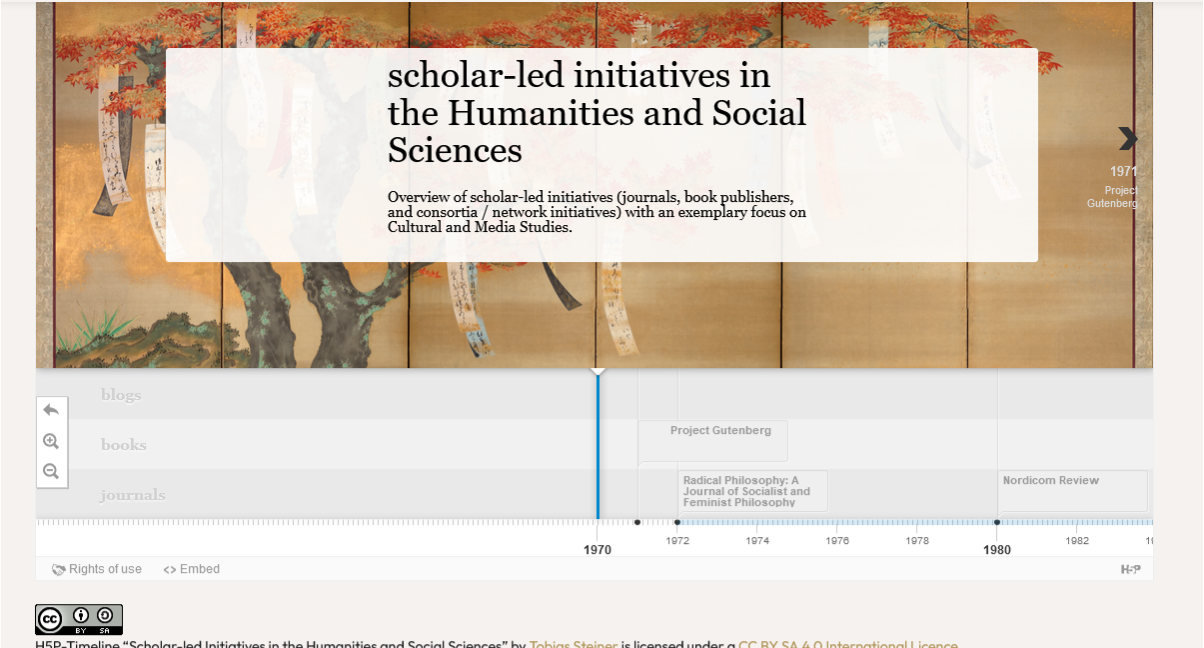
\includegraphics[width=0.9\textwidth]{img/abb2.png}
\caption{Abbildung 2: Interaktive Zeitleiste: scholar-led Initiativen
aus den Sozial- und Geisteswissenschaften der letzten fünf Jahrzehnte,
mit einem Fokus auf Medien- und Kulturwissenschaften. Abrufbar unter
\url{https://flavoursofopen.science/scholar-led-initiatives-history-and-recent-examples-from-cultural-and-media-studies/}}
\end{figure}

Zudem ist die Rolle, die einzelne Personen und durch aktiven Austausch
geformte Netzwerk-Kollektive in der Bildung der hier genannten
Communities spielen, deutlich herauszustellen: Oft werden in scholar-led
Projekten und Initiativen nicht mehr als ein oder zwei Kernakteur*innen
initial in einem bestimmten Bereich tätig und sorgen durch
kontinuierliche, oftmals aufwendige und zumeist unentgeltliche, in der
Freizeit beziehungsweise neben dem Hauptberuf stattfindende Netzwerk-
und Redaktionsarbeit dafür, dass sich Projekte langsam etablieren,
Publikationskanäle kontinuierlich betrieben und Ideen weiterentwickelt
werden können. Häufig formen sich daraus dann auch organisch weitere
Communities und scholar-led Projekte.

Erfreulicherweise sind erste Schritte einer Anerkennung dieser enormen
Leistung langsam auch auf der großen Policy-Ebene zu erkennen. So
widmeten sich beispielsweise Coalition S und Science Europe mit der 2021
veröffentlichten und seither vielbeachteten Studie zu
\href{https://www.coalition-s.org/diamond-unearthed-shining-light-on-community-driven-open-access-publishing/}{OA
Diamond Journals} dem Feld der non-profit Journals, die keine auf
Autor*innen-fokussierenden Gebühren erheben. Die als Teil der Studie
durchgeführte Journal-Erhebung kam auf eine geschätzte Zahl zwischen
17.000 und 29.000 Diamond-OA-Zeitschriften. Der Anteil der darunter
subsumierten scholar-led Journals wurde nicht weiter beleuchtet; es ist
jedoch anzunehmen, dass dieser Anteil nicht unerheblich sein dürfte. Aus
Sicht von scholar-led Initiativen und deren Akteur*innen und Communities
sind die ersten Schritte in Richtung potentieller Unterstützung durchaus
begrüßenswert die mittels der Studie beigefügten
\href{https://doi.org/10.5281/zenodo.4562790}{Empfehlungen} signalisiert
und nun unter anderem mittels der 2023 gestarteten Horizon
Europe-Projekte \href{https://diamasproject.eu/}{DIAMAS} und
\href{https://www.craft-oa.eu/}{Craft-OA} realisiert werden sollen.
Allerdings schwingt von Seiten so mancher scholar-led Initiative
sicherlich auch eine gewisse Skepsis mit, da Angebote wie das in den
\href{https://doi.org/10.5281/zenodo.4562790}{Empfehlungen} genannte
\enquote{Diamond Publishing Capacity Center} einerseits durchaus nötige
Unterstützung bieten könnte, andererseits jedoch eben
Zentralisierungsbewegungen wie diese potentiell das
Unabhängigkeitsstreben und die daraus resultierende
publikationskulturelle Diversität, welche gerade für scholar-led
Communities eine wichtige Rolle spielt, gefährden könnte.

Pierre Mounier schrieb schon vor zehn Jahren: \enquote{It is true that
the debate on open access to research results {[}...{]} was focused
until now not on humanities monographs, but rather on journals, and
firstly in science.} (Mounier 2013) Eine Dekade später, im Jahr 2023,
scheint sich die Geschichte zu wiederholen -- wir sehen mit dem oben
genannten Diamond OA Report und dem dazugehörigen
\href{https://doi.org/10.5281/zenodo.6282403}{Action Plan} ähnliche
Tendenzen der Fokussierung auf Journals. Und auch die fortwährenden
Diskussionen um die Open-Access-Farbenlehre à la Gold, Green, Platinum,
Diamondund so weiter fokussierten zum 20-jährigen Bestehen der BOAI
weiterhin primär auf den Journalbereich. Auf der anderen Seite findet
die große Vielfalt insbesondere der in den Geistes- und
Sozialwissenschaften auch jenseits von Journals stattfindenden
Wissenschaftskommunikation -- angefangen von Buchpublikationen
einschließlich Sammelbänden und Open Textbooks/Open Educational
Resources (OER) über Forschungsnetzwerke und deren digitale Plattformen
bis hin zum vielfältigen Universum von Blogs, Podcasts, et cetera, in
welcher scholar-led Communities einen wichtigen Teil spielen --
weiterhin kaum Beachtung. Speziell für den Buchbereich können hier
Strategien wie beispielsweise der aus einer scholar-led Community heraus
entwickelte vernetzte Ansatz des
\href{https://doi.org/10.16997/wpcc.918}{Scaling Small}, der aktuell mit
dem im Mai 2023 gestarteten COPIM-Anschlussprojekt
\href{https://doi.org/10.21428/785a6451.39b2b1ea}{Open Book Futures}
realisiert wird, eine vielversprechende Alternative bieten.

Abschließend sei hier erneut hervorgehoben, dass \enquote*{Öffnung} für
scholar-led Initiativen oftmals weit mehr als die bloße Verfügbarmachung
wissenschaftlichen Outputs im Sinne von \enquote*{klassischem} Open
Access bedeutet: Vielmehr werden in den Communities vielfach anhand
kontinuierlich praktizierter kritisch-konstruktiver Selbstreflexion
eigener Theorie und Praxis wichtige Fragen darüber neu verhandelt, auf
welche Art und Weise wir Wissenschaftskommunikation im digitalen Raum
betreiben wollen. Oder, wie Gary Hall schreibt: \enquote{How do you
apply your theoretical principles to the structures that make your work
visible?}
(\href{https://mitpress.mit.edu/9780262034401/pirate-philosophy/}{Hall,
2016}) Der daraus resultierende, von Adema und Hall beschriebene
\enquote{continuous struggle and critical Resistance}
(\href{https://doi.org/10.3898/NewF.78.07.2013}{Adema \& Hall, 2013}),
also die kontinuierliche Aushandlung der eigenen Positionierung
gegenüber hegemonialen Auslegungen von Open Access, der vielen der hier
vorgestellten scholar-led Initiativen als Kernmotivation dient, ist
meines Erachtens ein höchst wichtiger Aspekt und Grundpfeiler des
Strebens nach Offenheit in Wissenschaft und Forschung, der bisher im
breiten Diskurs zu Open Access leider gerne zugunsten Technik- oder
Policy-fokussierter Partikulardebatten vergessen wird. Gerade aus diesem
Grund verdienen scholar-led Projekte, Initiativen und Communities --
sowie insbesondere die sie konstitutierenden Akteur*innen -- die
Anerkennung sowie Unterstützung von allen im Wissenschaftssystem tätigen
Personen und Institutionen.

\hypertarget{referenzen}{%
\section{Referenzen}\label{referenzen}}

\emph{Eine erweiterte Auswahl von in diesem Beitrag zitierter sowie
relevanter Literatur ist in der offenen
\href{https://www.zotero.org/groups/2346073/open_research_open_science_open_scholarship/collections/9L48YBXU}{Zotero-Collection
\enquote{scholar-led publishing}} zur eigenen Weiternutzung verfügbar.}

Abrahamsson, Sebastian, Uli Beisel, Endre Dányi, Joe Deville, and Julien
McHardy. 2013. \enquote*{Mattering Press: New Forms of Care for STS
Books}. \emph{The EASST Review} 32 (4).
\url{https://www.easst.net/easst-review-volume-32-4-december-2013/mattering-press-new-forms-of-care-for-sts-books/}.

Adema, Janneke. 2009. \enquote*{Where Open Philosophy Meets Open Music}.
\emph{OPEN REFLECTIONS} (Blog). 23 June 2009.
\url{https://openreflections.wordpress.com/2009/06/23/where-open-philosophy-meets-open-music/}.

Adema, Janneke 2015. \enquote*{Knowledge Production Beyond The Book?
Performing the Scholarly Monograph in Contemporary Digital Culture}.
Coventry: Coventry University.
\url{https://web.archive.org/web/20181102223636/https://curve.coventry.ac.uk/open/file/8222ccb2-f6b0-4e5f-90de-f4c62c77ac86/1/ademacomb.pdf}.

Adema, Janneke. 2021a. \emph{Living Books: Experiments in the
Posthumanities}. Leonardo. Cambridge, MA, USA: MIT Press.

Adema, Janneke. 2021b. \enquote*{Toward a Diffractive Genealogy of Book
History}. In \emph{Living Books}, by Janneke Adema, 41--70. The MIT
Press. \url{https://doi.org/10.7551/mitpress/11297.003.0005}.

Adema, Janneke, Bowie, Simon, Mars, Marcell, and Steiner, Tobias. 2022.
\enquote*{Books Contain Multitudes: Exploring Experimental Publishing
(2022 Update)}. Community-led Open Publication Infrastructures for
Monographs (COPIM). \url{https://doi.org/10.5281/zenodo.6545475}.

Adema, Janneke, and Gary Hall. 2013. \enquote*{The Political Nature of
the Book: On Artists} Books and Radical Open Access'. \emph{New
Formations} 78 (78): 138--156.
\url{https://doi.org/10.3898/NewF.78.07.2013}. (OA-Version:
\url{https://pureportal.coventry.ac.uk/en/publications/the-political-nature-of-the-book-on-artists-books-and-radical-ope-2})

Adema, Janneke, and Samuel Moore. 2021. \enquote*{Scaling Small; Or How
to Envision New Relationalities for Knowledge Production}.
\emph{Westminster Papers in Communication and Culture} 16 (1).
\url{https://doi.org/10.16997/wpcc.918}.

Adema, Janneke, and Samuel A. Moore. 2017. \enquote*{The Radical Open
Access Collective: Building Alliances for a Progressive, Scholar-Led
Commons}. Online resource. \emph{Impact of Social Sciences Blog}. London
School of Economics and Political Science. 27 October 2017.
\url{http://blogs.lse.ac.uk/impactofsocialsciences/}.

Adema, Janneke. 2018. \enquote*{Collectivity and Collaboration:
Imagining New Forms of Communality to Create Resilience in Scholar-Led
Publishing}. \emph{Insights} 31 (0): 3.
\url{https://doi.org/10.1629/uksg.399}.

Adema, Janneke, and Graham Stone. 2017. \enquote*{Changing Publishing
Ecologies: A Landscape Study of New University Presses and Academic-Led
Publishing}. Zenodo. \url{https://doi.org/10.5281/zenodo.4420993}.

Adema, Janneke, and Tobias Steiner. 2023. \enquote*{Community-Led Open
Publication Infrastructures for Monographs: Final Report}. Zenodo.
\url{https://doi.org/10.5281/zenodo.7961527}.

Aguado López, Eduardo, and Arianna Becerril García. 2019.
\enquote*{Latin America's Longstanding Open Access Ecosystem Could Be
Undermined by Proposals from the Global North \textbar{} LSE Latin
America and Caribbean}. \emph{LSE Latin America and Caribbean Blog}. 6
November 2019.
\url{https://blogs.lse.ac.uk/latamcaribbean/2019/11/06/latin-americas-longstanding-open-access-ecosystem-could-be-undermined-by-proposals-from-the-global-north/}.

Becerril, Arianna, Jeroen Bosman, Lars Bjørnshauge, Jan Erik Frantsvåg,
Bianca Kramer, Pierre-Carl Langlais, Pierre Mounier, Vanessa Proudman,
Claire Redhead, and Didier Torny. 2021. \enquote*{OA Diamond Journals
Study. Part 2: Recommendations}. Zenodo.
\url{https://doi.org/10.5281/zenodo.4562790}.

Becerril-García, Arianna, and Eduardo Aguado-López. 2018. \enquote*{The
End of a Centralized Open Access Project and the Beginning of a
Community-Based Sustainable Infrastructure for Latin America:
Redalyc.Org after Fifteen Years The Open Access Ecosystem in Latin
America}. In \emph{ELPUB 2018}, edited by Leslie Chan and Pierre
Mounier. Vol. Connecting the Knowledge Commons: From Projects to
Sustainable Infrastructure. Toronto, Canada: Association Francophone
d'Interaction Homme-Machine (AFIHM).
\url{https://doi.org/10.4000/proceedings.elpub.2018.27}.

Bollier, David. 2022'The Radical Open Access Collective: Building Better
Knowledge Commons'. Frontiers of Commoning. (Blog). 31 March 2022.
\url{https://www.bollier.org/blog/radical-open-access-collective-building-better-knowledge-commons}.

\emph{Books Contain Multitudes: Exploring Experimental Publishing (2022
Update)}. 2022. Community-led Open Publication Infrastructures for
Monographs (COPIM). \url{https://doi.org/10.21428/785a6451.1792b84f}.

Cabrerizo, Franco M. 2022. \enquote*{Open Access in Low-Income Countries
--- Open Letter on Equity}. \emph{Nature} 605 (7911): 620--620.
\url{https://doi.org/10.1038/d41586-022-01414-7}.

Chan, Leslie, Darius Cuplinskas, Michael Eisen, Fred Friend, Yana
Genova, Jean-Claude Guédon, Melissa Hagemann, et al.~2002.
\enquote*{Budapest Open Access Initiative: Declaration}. \emph{BOAI}
(Blog). 14 February 2002.
\url{https://www.budapestopenaccessinitiative.org/read/}.

COPIM. 2023. \enquote*{£5.8 Million Funding to Significantly Expand and
Accelerate COPIM Open Access Infrastructures}. \emph{Community-Led Open
Publication Infrastructures for Monographs (COPIM)}, March.
\url{https://doi.org/10.21428/785a6451.39b2b1ea}.

COUNTERPRESS. \enquote*{About}. Accessed 11 June 2023.
\url{https://counterpress.org.uk/about/}.

Crawford, Walt. 2002. \enquote*{Free Electronic Refereed Journals:
Getting Past the Arc of Enthusiasm}. \emph{Learned Publishing} 15 (2):
117--123. \url{https://doi.org/10.1087/09531510252848881}.

Deppe, Arvid, and Daniel Beucke. 2017. \enquote*{Urspünge und
Entwicklung von Open Access}. In Söllner, Konstanze / Mittermaier,
Bernhard (Hrsg.): Praxishandbuch Open Access (S. 12--20). De Gruyter
Saur. Akzeptiertes Manuskript via Zenodo.
\url{https://doi.org/10.5281/ZENODO.802639}.

Deville, Joe. 2016. \enquote*{Open Access Publishing and the Future of the University}. \emph{Mattering Press Blog} . 29 September 2016. \url{https://www.matteringpress.org/blog/open-access-publishing-and-the-future-of-the-university}.

Deville, Joe, Jeroen Sondervan, Graham Stone, and Sofie Wennström. 2019.
\enquote*{Rebels with a Cause? Supporting Library- and Academic-Led Open
Access Publishing}. \emph{LIBER Quarterly} 29 (1): 1--28.
\url{https://doi.org/10.18352/lq.10277}.

Eve, Martin Paul. 2013. \enquote*{Open Access, \enquote{Neoliberalism}, \enquote{Impact} and the Privatisation of Knowledge}. \emph{Martin Paul Eve} (Blog). 10 March 2013. \url{https://eve.gd/2013/03/10/open-access-neoliberalism-impact-and-the-privatisation-of-knowledge/}.

Fathallah, Judith. 2023. \enquote*{Governing Scholar-Led OA Book
Publishers: Values, Practices, Barriers}. \emph{Community-Led Open
Publication Infrastructures for Monographs (COPIM)}, April.
\url{https://doi.org/10.21428/785a6451.e6fcb523}.

Franssen, Thomas, and Paul Wouters. 2017. \enquote*{Science and Its
Significant Other: Representing the Humanities in Bibliometric
Scholarship}. \url{https://doi.org/10.48550/ARXIV.1710.04004}.

Ganz, Kathrin, Marcel Wrzesinski, and Markus Rauchecker. 2019.
\enquote*{Nachhaltige Qualitätssicherung und Finanzierung von non-APC,
scholar-led Open-Access-Journalen}.
\url{https://doi.org/10.18452/21418}.

\enquote*{Geschichte des Open Access}. 2023. \emph{Open-Access.Network}
(Blog). 25 April 2023.
\url{https://open-access.network/informieren/open-access-grundlagen/geschichte-des-open-access}.

Grigar, Dene, Nicholas Schiller, Vanessa Rhodes, Mariah Gwin, Veronica
Whitney, and Katie Bowen. 2018. \enquote*{Rebooting Electronic Literature: Photos of David Kolb's \enquote{Socrates in the Labyrinth}}.
In \emph{Rebooting Electronic Literature: Documenting Pre-Web Born
Digital Media}. Vol. 1. Electronic Literature Lab.
\url{https://scalar.usc.edu/works/rebooting-electronic-literature/photos-of-david-kolbs-socrates-in-the-labyrinth}.

Hall, Gary. 2003a. \enquote*{Cultural Studies E-Archive Project
(Original Pirate Copy)}. \emph{Culture Machine} (Blog). 14 January 2003.
\url{https://culturemachine.net/the-e-issue/cultural-studies-e-archive-project/}.

Hall, Gary. 2003b. \enquote*{Cultural Studies E-Archive Project
(Original Pirate Copy)}. \emph{Culture Machine} 5 (January).
\url{https://culturemachine.net/the-e-issue/cultural-studies-e-archive-project/}.

Hall, Gary. 2008. \emph{Digitize This Book!\,: The Politics of New
Media, or Why We Need Open Access Now}. Electronic Mediations 24.
Minneapolis: University of Minnesota Press.

Hall, Gary. 2015. \enquote*{Open Humanities Press: Funding and
Organisation}. \emph{Media Gifts} (Blog). 13 June 2015.
\url{http://garyhall.squarespace.com/journal/2015/6/13/open-humanities-press-funding-and-organisation.html}.

Hall, Gary. 2016. \emph{Pirate Philosophy for a Digital Posthumanities}.
Leonardo Book Series. Cambridge, Massachusetts: The MIT Press.
\url{https://doi.org/10.7551/mitpress/10463.001.0001}.

Harnad, Stevan. 1991. \enquote*{Post-Gutenberg Galaxy: The Fourth
Revolution in the Means of Production of Knowledge}.
\url{https://hdl.handle.net/10657/5147}\href{https://uh-ir.tdl.org/handle/10657/5147}{.}

Harnad, Stevan. 1995. \emph{Scholarly Journals at the Crossroads: A
Subversive Proposal for Electronic Publishing}. Edited by Anna Shumelda
Okerson and James J. O'Donnell. Association of Research Libraries.
\url{https://eprints.soton.ac.uk/362894/}.

Harnad, Stevan. 2003. \enquote*{For Whom the Gate Tolls? How and Why to
Free the Refereed Research Literature Online Through Author/Institution
Self-Archiving, Now}.
\url{https://web.archive.org/web/20171105224125/http://users.ecs.soton.ac.uk/harnad/Tp/resolution.htm}.

Harnad, Stevan. 1999. \enquote*{The Future of Scholarly Skywriting}.
Accessed 19 February 2022.
\url{https://www.southampton.ac.uk/~harnad/Papers/Harnad/harnad99.aslib.html}.

Hole, Brian, Chris Land, Craig Saper, Eileen A. Joy, Joe Deville,
Kathleen Fitzpatrick, Martin Paul Eve, et al.~2017. Interview
transcriptions\,: Changing Publishing Ecologies. A Landscape Study of
New University Presses and Academic-led Publishing Interview by Janneke
Adema. \url{https://repository.jisc.ac.uk/6652/}.

Joy, Eileen A. 2020. \enquote*{Not Self-Indulgence, but
Self-Preservation: Open Access and the Ethics of Care}, October.
\url{https://doi.org/10.7551/mitpress/11885.003.0032}.

Julien McHardy {[}@hardyjuls{]}. 2020. \enquote*{2/ We Started the
Scholar-Led Press @matteringpress Because Our Field of Science and
Technology Studies, for All Its Critical Knowledge \& Infrastructure
Studies Lacked engagement and Experimentation with Scholarly
Publishing. Https://Mat teringpress.Org/Books}. Tweet. \emph{Twitter}.
\url{https://twitter.com/hardyjuls/status/1314347568185462786}.

Kamerlin, Shina Caroline Lynn, David J. Allen, Bas de Bruin, Etienne
Derat, and Henrik Urdal. 1970. \enquote*{Journal Open Access and Plan S:
Solving Problems or Shifting Burdens?} \emph{Development and Change} n/a
(n/a). \url{https://doi.org/10.1111/dech.12635}.

Kember, Sarah. 2014a. \enquote*{Opening Out from Open Access: Writing
and Publishing in Response to Neoliberalism}.
\url{https://doi.org/10.7264/N31C1V51}.

Kember, Sarah. 2014b. \enquote*{Why Write? Feminism, Publishing and the
Politics of Communication}. \emph{New Formations} 83 (83): 99--116.
\url{https://doi.org/10.3898/NEWF.83.06.2014}.

Kiesewetter, Rebekka. 2020. \enquote*{Undoing Scholarship: Towards an
Activist Genealogy of the OA Movement}. \emph{Tijdschrift voor
Genderstudies} 23 (2): 113--130.
\url{https://doi.org/10.5117/TVGN2020.2.001.KIES}.

Knöchelmann, Marcel. 2020. \enquote*{The Democratisation Myth: Open
Access and the Solidification of Epistemic Injustices}. Preprint.
SocArXiv. \url{https://doi.org/10.31235/osf.io/hw7at}.

Laporte, Steven. 2016. \enquote*{Preprint for the Humanities - Fiction
or a Real Possibility?} Preprint. SocArXiv.
\url{https://doi.org/10.31235/osf.io/jebhy}.

Masterman, Eleanor. 2020. \enquote*{\enquote{Communists of Knowledge}? A Case for the Implementation of \enquote{Radical Open Access} in the Humanities and Social Sciences}.
\url{http://dx.doi.org/10.17613/t5n3-x550}.

Mitchell, William J. 1996. \enquote*{Homer to Home-Page: Designing
Digital Books}. February 1996.
\url{http://mitpress2.mit.edu/e-books/City_of_Bits/Text_Unbound/text_unbound.html}.

Moore, Samuel. 2019. \enquote*{Common Struggles: Policy-Based
vs.~Scholar-Led Approaches to Open Access in the Humanities}.
\url{http://dx.doi.org/10.17613/st5m-cx33}.

Moore, Samuel A. 2020. \enquote*{Revisiting \enquote{the 1990s Debutante}: Scholar-led Publishing and the Prehistory of the Open Access Movement}. \emph{Journal of the Association for Information Science and Technology} 71 (7): 856--66. \url{https://doi.org/10.1002/asi.24306}. (Preprint: \href{https://hcommons.org/deposits/item/hc:24075}{http://dx.doi.org/10.17613/gty2-w177})

Moore, Samuel A. 2021. \enquote*{Open Access, Plan S and
\enquote{Radically Liberatory} Forms of Academic Freedom}.
\emph{Development and Change}, January, dech.12640.
\url{https://doi.org/10.1111/dech.12640}.

Moore, Samuel A. 2017. \enquote*{A Genealogy of Open Access:
Negotiations between Openness and Access to Research}. \emph{Revue
Française Des Sciences de l'information et de La Communication}, no. 11
(August). \url{https://doi.org/10.4000/rfsic.3220}.

Moore, Samuel A.. 2019. \enquote*{Open *By* Whom? On the Meaning of
\enquote{Scholar-Led}}. \emph{Samuel Moore} (Blog). 24 October 2019.
\url{https://www.samuelmoore.org/2019/10/24/open-by-whom-on-the-meaning-of-scholar-led/}.

Mounier, Pierre. 2013. \enquote*{« The Book Is a Conversation ».
Really\,?} \emph{Blogo Numericus} (Blog). 16 July 2013.
\url{https://web.archive.org/web/20130716140044/http://blog.homo-numericus.net:80/article11208.html}.

Okerson, Anna Shumelda. 1994. \enquote*{Oh Lord, Won't You Buy Me A
Mercedes Benz Or, There Is a There There}. \emph{Surfaces} IV (102):
Folio 1. \url{https://doi.org/10.7202/1064955ar}.

Olleros, F. Xavier. 2018. \enquote*{Antirival Goods, Network Effects and
the Sharing Economy}. \emph{First Monday}, February.
\url{https://doi.org/10.5210/fm.v23i2.8161}.

Parikka, Jussi. 2014. \enquote*{A Mini-Interview: Mercedes Bunz Explains
Meson Press}. \emph{Machinology} (Blog). 11 July 2014.
\url{https://jussiparikka.net/2014/07/11/a-mini-interview-mercedes-bunz-explains-meson-press/}.

Projekt AurOA. 2022. \enquote*{Publizieren und Open Access in den
Geisteswissenschaften: Erkenntnisse aus dem Projekt AuROA zu den
Stakeholdern im Publikationsprozess}. Essen.
\url{https://projekt-auroa.de/wp-content/uploads/2022/03/AuROA-Publizieren-und-Open-Access-in-den-Geisteswissenschaften.pdf}.

Raju, Reggie, and Jill Claassen. 2022. \enquote*{Open Access: From Hope
to Betrayal}. \emph{College \& Research Libraries News} 83 (4): 161.
\url{https://doi.org/10.5860/crln.83.4.161}.

Schalkwyk, François van, Joe Deville, Jeff Pooley, Mercedes Bunz,
Alessandra Tosi, and Eileen A. Joy. 2023. Governing Scholar-Led OA Book
Publishers: Interviews with Presses Interview by Judith Fathallah.
\url{https://doi.org/10.5281/zenodo.7816845}.

Steiner, Tobias. 2022. \enquote*{Old Traditions: Scholar-led publishing
und Open Access --- zu den Anfängen digitalen scholar-led Publishings in
den Geistes- und Sozialwissenschaften (Teil 2)}. \emph{Open Media
Studies} (Blog). 26 August 2022.
\url{https://mediastudies.hypotheses.org/3324}.

Strangelove, Michael. 1992. \enquote*{EJOURNL1 DIRECTRY: Electronic
Journals and Newsletters}.
\url{http://info.cern.ch/hypertext/DataSources/Journals.html}.

Suber, Peter. 2016. \enquote*{Knowledge as a Public Good}. In
\emph{Knowledge Unbound: Selected Writings on Open Access, 2002--2011}.
MIT Press.
\url{https://knowledgeunbound.mitpress.mit.edu/pub/cjktrtqe/release/1}.

Steiner, Tobias (2023) Lost in translation? Revisiting notions of
community- and scholar-led publishing in international contexts.
ScholarLed Blog, 4 July 2023.
\url{https://blog.scholarled.org/lost-in-translation-revisiting-notions-of-community-and-scholar-led-publishing-in-international-contexts/}

Tennant, Jonathan, Ritwik Agarwal, Ksenija Baždarić, David Brassard, Tom
Crick, Daniel J. Dunleavy, Thomas Rhys Evans, et al.~2020. \enquote*{A
Tale of Two \enquote{Opens}: Intersections between Free and Open Source
Software and Open Scholarship}. Preprint. SocArXiv.
\url{https://doi.org/10.31235/osf.io/2kxq8}.

\enquote*{The Budapest Open Access Initiative: 20th Anniversary
Recommendations}. 2022. \emph{BOAI} (Blog). Accessed 2 June 2023.
\url{https://www.budapestopenaccessinitiative.org/boai20/}.

Treloar, Andrew. 1996. \enquote*{Better than Print? Hypermedia Scholarly
Publishing and the World Wide Web}. In \emph{Andrew Treloar: Blog}.
Melbourne.
\url{https://andrew.treloar.net/research/publications/vala96/index.html}.

%autor
\begin{center}\rule{0.5\linewidth}{0.5pt}\end{center}

\textbf{Tobias Steiner} hat in Hamburg und London studiert und hält
einen Master of Arts in Television Studies. Seit 2011 ist er in
Open-Scholarship-Projekten aktiv, koordinierte gemeinsam mit Janneke
Adema und Gary Hall zwischen 2020 und 2023 in der Rolle des
Projektmanagers das internationale Infrastruktur-Verbundprojekt
\href{https://www.copim.ac.uk}{Community-Led Open Publication
Infrastructures for Monographs} (COPIM) und ist seit Juni 2023
Produktmanager beim COPIM-Spinoff \href{https://thoth.pub/}{Thoth Open
Metadata}. Seit 2013 ist Tobias in seiner Freizeit zudem Co-Editor von
\href{https://cstonline.net/}{CSTOnline}, des offenen scholar-led Blogs
von \emph{Critical Studies in Television}, hat 2016 das
\href{http://ffk-journal.de/}{Journal des Film- und
Fernsehwissenschaftlichen Kolloquiums} technisch mitinitiiert, ist
Mitglied des \href{https://radicaloa.disruptivemedia.org.uk/}{Radical
Open Access Collective}, und Mitautor des
\href{https://graphite.page/scholar-led-manifest/}{scholar-led.network-Manifests}
(Deutsch 2021,
\href{https://graphite.page/scholar-led-manifesto/}{English version}
2022). Seine ORCiD:
\href{https://orcid.org/0000-0002-3158-3136}{0000-0002-3158-3136}.

\end{document}